%
%TODOs
% * Try-catch
% Functions måste vara mer grundläggande förklarat. Gör avsnittet längre.
% Kodexempel för varje sektion
% Algoritm begreppbox
% Beskriv vad sortering är tydligare
% Kapitel två överlag lite för otydligt

\documentclass[a4paper]{book}

\usepackage[a4paper, margin=1.5cm]{geometry}

% Paket
\usepackage[utf8]{inputenc} % Svensk teckenstandard
\usepackage[swedish]{babel} % Språkpaket
\usepackage{amsmath, amssymb} % För matematik
\usepackage{listings} % Kodblock
\usepackage{xcolor} % Färg för kod
\usepackage[dvipsnames]{xcolor}


% För xsim (Excersice and solution)
\usepackage{amssymb}
\usepackage[use-files]{xsim}
\usepackage{lipsum,hyperref}


% För dyslexi
% Ställ in typsnitt och grundinställningar
\usepackage{fontspec}
\setmainfont{Arial}[LetterSpace=8]
\renewcommand{\baselinestretch}{1.5} % Sätt radavstånd till 1,5
\setlength{\spaceskip}{1.2em plus 0.2em minus 0.2em} % Ordavstånd
\raggedright

% För textrutor
\usepackage[most]{tcolorbox}



\newtcolorbox[auto counter, number within=section]{rconceptbox}[2][]{
    size=small,
    sharp corners,
    right=1cm,
    colframe=orange,
    colback=orange!10,
    coltitle=black,
%    floatplacement=ht,float,
    title=#2,
    before=\vspace{1em}, % Mellanrum ovanför rutan
    after=\vspace{1em},  % Mellanrum under rutan
    #1,
}

\newtcolorbox{outputbox}[2][]{
    size=small,
    sharp corners,
    right=1cm,
%    colframe=gray!10,
    colback=blue!5,
    coltitle=blue!10,
%    floatplacement=ht,float,
    title=#2,
    before=\vspace{1em}, % Mellanrum ovanför rutan
    after=\vspace{1em},  % Mellanrum under rutan
    #1,
}


\newtcolorbox{observerabox}[1][]{
    size=small,
    sharp corners,
    right=1cm,
    colframe=OliveGreen,
    colback=OliveGreen!10,
    coltitle=black,
    title=Observera!,
    before=\vspace{1em}, % Mellanrum ovanför rutan
    after=\vspace{1em},  % Mellanrum under rutan
    #1,
}

\newtcolorbox{refbox}[1][]{
    size=small,
    sharp corners,
    right=1cm,
    colframe=Blue,
    colback=Blue!10,
    coltitle=black,
    before=\vspace{1em}, % Mellanrum ovanför rutan
    after=\vspace{1em},  % Mellanrum under rutan
    #1,
}

\lstset{
    literate={å}{{\r{a}}}1
             {ä}{{\"a}}1
             {ö}{{\"o}}1
             {Å}{{\r{A}}}1
             {Ä}{{\"A}}1
             {Ö}{{\"O}}1
}
% Anpassa utseendet på kod
\lstset{
    basicstyle=\ttfamily\small,
    keywordstyle=\color{blue},
    commentstyle=\color{green!50!black},
    stringstyle=\color{red},
    backgroundcolor=\color{gray!10},
    frame=single,
    numbers=left,
    numberstyle=\tiny\color{gray},
    breaklines=true,
    resetmargins=true,
    captionpos=b,
    language=Python,
    showstringspaces=false,
    tabsize=2,
    upquote=true,
    floatplacement=ht,float
}

\newcommand{\begrepp}[2]{
	\begin{rconceptbox}{#1}#2\end{rconceptbox}
}
\newcommand{\observera}[1]{
	\begin{observerabox}{}#1\end{observerabox}
}
\newcommand{\pythonoutput}[2]{
	\begin{outputbox}{#1}#2 \end{outputbox}
}
\newcommand{\exToSecRef}[1]{
Exempel från avsnitt \ref{#1}.
}
\newcommand{\secToExRef}[1]{
\begin{refbox}För fler kodexempel se appendix \ref{#1}\end{refbox}
}


\title{Programmering 1 med Python}
\author{Patrik Berggren}

\hypersetup{colorlinks}

\DeclareExerciseHeadingTemplate{custom}
  {\section{\XSIMexpandcode{\XSIMtranslate{default-heading}}}}

\DeclareExerciseEnvironmentTemplate{custom}
  {%
    \IfInsideSolutionTF
      {\label{sol:\ExerciseID}}
      {\label{ex:\ExerciseID}}%
    \paragraph*
      {%
        \XSIMmixedcase{\GetExerciseName}%
        \IfInsideSolutionTF
          {
            till \GetExerciseParameter{exercise-name}%
            ~\GetExerciseProperty{counter}%
            ~(Från sida~\pageref{ex:\ExerciseID})
          }
          {%
            ~\GetExerciseProperty{counter}%
%            \GetExercisePropertyT{subtitle}{~(\PropertyValue)}
          }
      }
      \noindent
  }
  {%
    \IfInsideSolutionF
      {\par\leavevmode\hfill
       Lösningar på sida~\pageref{sol:\ExerciseID}~$\blacktriangleleft$}%
  }
\xsimsetup{
  exercise/name = Uppgift,
  solution/name = Lösning,
  exercise/template = custom ,
  solution/template = custom ,
  print-solutions/headings-template = custom
}
\DeclareExerciseHeadingTemplate{solution}{%
    \section{ Lösningsförslag}
}




%For flowcharts
\usepackage{tikz}
\usetikzlibrary{shapes.geometric, arrows}

\tikzstyle{startstop} = [rectangle, rounded corners, 
minimum width=3cm, 
minimum height=1cm,
text centered, 
draw=black, 
fill=red!30]

\tikzstyle{io} = [trapezium, 
trapezium stretches=true, % A later addition
trapezium left angle=70, 
trapezium right angle=110, 
minimum width=3cm, 
minimum height=1cm, text centered, 
draw=black, fill=blue!30]

\tikzstyle{process} = [rectangle, 
minimum width=3cm, 
minimum height=1cm, 
text centered, 
text width=3cm, 
draw=black, 
fill=orange!30]

\tikzstyle{decision} = [diamond, 
minimum width=3cm, 
minimum height=1cm,
%yshift=-0.5cm,
aspect=3,
text centered, 
draw=black, 
fill=green!30]
\tikzstyle{arrow} = [thick,->,>=stealth]


%\includeonly{./sectionContent/sectionFlowchart}
%\includeonly{./sectionExamples/sectionFlowchart}

\begin{document}

% Titelsida
\maketitle
\tableofcontents

\chapter{Introduktion}
\label{chapter:intro}
Välkommen till denna bok om programmering med \textbf{Python}. Här lär du dig de grundläggande byggstenarna för att skriva och förstå kod. Vi går steg för steg med enkla exempel och övningar. 

Kom ihåg att stanna upp och läs igen om du inte är säker på om du förstått. 
Övningarna syftar till att kontrollera att man också själv kan använda det som avsnitten förklarar. 
I slutet på boken finns lösningsförslag på övningarna. 
I programmering kan det finnas många olika sätt att lösa en uppgift på. 
Lösningsförslagen är inte nödvändigtviss det ända eller ens det bästa sätten, men ett förslag på hur man kan tänka. 

\section{Kodexempel}
Förutom kodexempel i varje avsnitt finns också ett appendix med fler kodexempel.
Det kan vara bra att kolla på fler exempel för att se en större variation av användning av de programmeringskoncept vi kollar på i avsnitten.

\section{Vad är programmering?}
Programmering handlar om att skriva instruktioner som en dator kan förstå och följa. Python är ett av de mest populära programmeringsspråken eftersom det är lätt att läsa och använda. Det är också ett vanligt val inom maskininlärning, eller webbutveckling. 

\begrepp{Python}{Python är ett programmeringsspråk. Det används för att skapa allt från enkla program till avancerade system som spel och webbplatser.}


\newpage
\chapter{Grunder i programmering med python}
\label{chapter:1}

\section{Utskrifter med print}
\label{section:print}
\subsection{Hello World Program}
Ett av de första programmen man brukar skriva när man lär sig ett nytt programmeringsspråk är det så kallade ''hello world''-programmet. Det vill säga ett program som skriver ut texten \textbf{hello world} på skärmen. 
Så här ser det ut i Python:
\begin{lstlisting}[title=Hello World-program]
print("Hello, world!")
\end{lstlisting}

När du kör programmet visas texten \texttt{Hello, world!} i terminalen.

\begrepp{Terminal/Konsol}{En terminal (eller konsol) är ett program där du kan skriva in och köra kommandon, till exempel för att köra ditt Python-program. }

\subsection{Syntax i programmering}
När vi kör Hello World-programmet behöver datorn veta vad vi vill göra. 
Datorn kräver att vi skriver vårat program på ett väldigt exakt formatterat sätt, detta kallas syntax.
Exempelvis skulle programmet ovan inte gå att köra om vi hade gjort om det på något av sätten nedan där 
enstaka tecken tagits bort eller till och med om vi använder stora istället för små bokstäver.
\begin{lstlisting}[title=Felaktig syntax i kod]
PRINT("Hello, world")
Print("Hello, world")
print("Hello, world"
print("Hello, world)
print(Hello, world")
print(Hello, world)
print "Hello, world"
skrivut(Hello, world)
\end{lstlisting}

\begrepp{Syntax}{Syntax är reglerna som bestämmer hur kod ska skrivas för att datorn ska förstå den. Om vi bryter mot syntaxen, fungerar inte programmet.}
\begrepp{Syntax highlighting}{När våran editor färglägger olika delar av koden.
Det gör det enklare för oss att läsa kod, eller att se när syntaxen är fel som i exemplena ovan. }


\subsection{Funktionen \texttt{print()}}
Funktionen \texttt{print()} används för att skriva ut text eller resultat på skärmen. En funktion är en bit kod som utför en specifik uppgift. När vi använder en funktion, skickar vi in något den ska jobba med. Detta kallas ett \textbf{argument}.

Här är ett exempel:
\begin{lstlisting}[title=Syntax för print()]
print("Hej på dig")
\end{lstlisting}

- \textbf{print} är funktionens namn. \\
- \textbf{paranteser} kommer alltid efter namnet på en funktion. Inom parantesen skriver vi det vi skickar in i funktionen (Argumentet). Detta kan liknas vid funktionsbegreppet i matematik där vi ofta skriver f(x). Där är f namnet och x argumentet. \\
- \textbf{"Hej på dig"} är argumentet. Vi behöver markera för python att det vi skickat in är en text. Det gör vi genom att använda citattecken. Vi kommer senare att förstå varför. 

\begrepp{Funktion}{En funktion är en bit kod som gör en uppgift. Vi kan använda funktioner genom att anropa dem med deras namn.}

\begrepp{Argument}{Ett argument är något vi skickar in i en funktion, till exempel en text eller ett tal. Argument ges alltid inom ett par paranteser.}

\subsection{Programmering kan räkna ut saker}
Python kan användas för att göra matematiska beräkningar, till exempel addition, subtraktion, multiplikation och division. 
Här är några exempel:

\begin{lstlisting}[title=Matematik i Python]
print(5 + 3)  # Addition
print(10 - 4) # Subtraktion
print(7 * 2)  # Multiplikation
print(9 / 3)  # Division
\end{lstlisting}

\observera{I programmet ser du att vi skrivit förklaring till koden efter tecknet \#. 
Genom att använda \# tecknet kan vi tala om för python att det som kommer efter inte är kod utan en förklaring. 
Det kan vara bra för att den som läser koden ska förstå den. 
Vi kommer prata mer om kodkommentarer i ett senare avsnitt.}

När detta körs visas resultaten på skärmen:
\pythonoutput{Output från Matematik i Python - programmet}{
8 \\
6\\
14\\
3.0
}

\begrepp{Output}{Det som programmet skriver ut på skärmen}

\subsection{Övningar}
Här är några övningar för att testa det du har lärt dig.

\begin{exercise}
Skriv ett program som visar texten \texttt{Hej! Jag lär mig Python.} på skärmen.
\end{exercise}
\begin{solution}
\begin{lstlisting}
print("Hej! Jag lär mig Python.")
\end{lstlisting}

\end{solution}

\begin{exercise}
Använd funktionen \texttt{print()} för att visa resultaten av följande beräkningar: \\
12 + 5 \\
20 - 8 \\ 
4 * 3 \\
16 / 4 \\
\end{exercise}
\begin{solution}

\begin{lstlisting}
print(12 + 5)
print(20 - 8)
print(4 * 3)
print(16 / 4)
\end{lstlisting}

\pythonoutput{Output}{
17\\
12\\
12\\
4.0}

\end{solution}

\begin{exercise}
Skriv ett program som använder \texttt{print()} för att visa texten \textbf{Python är roligt!} och beräkningen \texttt{10 + 15} på olika rader.
\end{exercise}
\begin{solution}

\begin{lstlisting}
print("Python är roligt!")
print(10+15)
\end{lstlisting}

\end{solution}

\secToExRef{examples:print}


\newpage
\section{Variabler och Sekvensiell Exekvering}
\label{section:variables}
\subsection{Vad är en variabel?}
En variabel är som en namngiven låda där vi kan lagra data, som till exempel tal eller text. Vi kan senare ändra innehållet i lådan eller använda det i beräkningar.

\begin{lstlisting}[title=Tilldelning]
minvariabel = 100+1
\end{lstlisting}

I programmet ser vi hur vi sparar ett värde i en variabel. 
I exemplet heter våran variabel \textbf{minvariabel} och vi sparar värdet 101 i den.
Vi kan senare i programmet återanvända våran variabel för att hämta det värde vi sparat i den. 
Notera att vi använder likamedtecknet = men inte på samma sätt som i matematik. 
När python ser = så kommer den först göra en uträkning av det som står på höger sida. 
Det blir alltid ett konkret värde, exempelvis ett tal, eller en text. 
I exemplet räknar python ut åt oss att $100+1$ blir $101$. 
Python sparar sedan värdet $101$ i variabeln som vi döpt till \textbf{minvariabel}.

\begrepp{Likamedtecknet}{Likamedtecknet betyder i programmering att vi sparar värdet på högersidan i variabeln vi skrivit på vänstersidan.}
\observera{Likamedtecken i programmering betyder \textbf{INTE} samma sak som i matematik. Det kan se ut som att vi ställt upp en ekvation, 
men vi använder = bara för att spara ett uträknat värde.}


\subsection{Använda variabler}


\begin{lstlisting}[title=Exempel på variabler]
x = 5
y = 10
z = x + y
print(z)
\end{lstlisting}

När detta program körs, kommer resultatet \texttt{15} att visas på skärmen eftersom \texttt{x} är 5 och \texttt{y} är 10.

\begrepp{Variabel}{En plats i datorns minne där data, som tal eller text, lagras. Vi ger platsen ett namn för att enkelt kunna använda den i programmet.}

\subsection{Datatyper}
Data i Python kan ha olika typer, som bestämmer vad vi kan göra med den. 
Några vanliga typer:\\
- \texttt{int}: Heltal (till exempel \texttt{5})\\
- \texttt{float}: Decimaltal (till exempel \texttt{3.14})\\
- \texttt{str}: Text, även kallad sträng (till exempel \texttt{"Hej!"})\\

\begin{lstlisting}[title=Exempel på olika datatyper]
tal = 5           # int
decimaltal = 3.14 # float
text = "Hej!"     # str
\end{lstlisting}

Eftersom datorn bara ser 1:or och 0:or i minnet behöver den hålla reda på om det vi sparat
är ett heltal eller en text. Vi kommer gå djupar kring datatyper senare, men nu vet du varför vi behöver citattecken när vi 
skriver en text. 
Datatyper är också förklaringen till varför \texttt{print(4/2)} blir 2.0 och inte 2. 
Python gör nämligen om alla divisioner till float (decimaltal).


\begrepp{Datatyp}{En typ av värde, exempelvis heltal (integer), eller textvärden (string)}
\begrepp{Integer}{Variabler av datatypen integer (förkortat int) innehåller heltalsvärden}
\begrepp{Float}{Variabler av datatypen float innehåller decimaltal}
\begrepp{String}{Variabler av datatypen string (förkortat str) innehåller textvärden. På svenska säger vi också att datatypen är en sträng.}

\subsection{Sekvensiell exekvering}
När ett program körs, läses koden rad för rad, uppifrån och ned. 
Detta kallas sekvensiell exekvering. 
Ordningen på kod spelar alltså mycket stor roll!!!
Här är ett exempel:

\begin{lstlisting}[title=Ordning i koden spelar roll]
x = 5
print(x)
x = 7
print(x)
\end{lstlisting}

Resultatet blir först \texttt{5} och sedan \texttt{7}, eftersom värdet på \texttt{x} ändras innan den skrivs ut andra gången.

\begrepp{Exekvering}{
Exekvering betyder att man kör programmeringskod. 
Det vill säga att datorn steg för steg går igenom koden och utför våra instruktioner.}

\begin{minipage}{\linewidth}
\begin{lstlisting}[title=Användning av samma variabel två gånger]
x = 5
print(x)
x = x+2
print(x)
\end{lstlisting}
\end{minipage}

Detta program skriver också ut 5 och sen 7. 
Det beror på att raden x=x+2 betyder att vi först räknar ut högersidan, 
vilket blir 5+2 eftersom x, när programmet ska köra rad 3, har värdet 5. 
Vi sätter sedan detta värde som nytt värde på variabeln x.
Det går med andra ord bra att spara ett nytt värde i en variabel som beror på det gamla värdet.
Det är också ganska vanligt att man vill göra just det, exempelvis för att öka en variabels värde med Ett, 
vilket vi alltså kan åstadkomma genom \texttt{x=x+1}.

\subsection{Strängkonkatenering}
Om vi har sparat textvärden, det vill säga strängar, i våra variabler kan vi sätta ihop texterna med + tecknet.
Detta kallas konkatenering.

\begin{lstlisting}[title=Konkatenering av strängar]
namn = "Kalle"
efternamn = "Anka"
hela = namn + efternamn
print(hela)
\end{lstlisting}
\pythonoutput{Output}{KalleAnka}

I programmet ser vi att + tecknet används också för texter för att konkatenera eller slå ihop dom. 
Vi sparar resultatet i en ny variabel vi döpt till hela, som vi sedan skriver ut med \texttt{print(hela)}.
Vi hade också kunnat addera textsträngarna direkt med \texttt{print("Kalle"+\string"Anka")}.

\begrepp{Konkatenering}{Konkatenering av texter betyder att vi sätter ihop texterna direkt efter varandra. Konkatenering av texten \textbf{hej} och texten \textbf{då} blir \textbf{hejdå}.}

\subsection{Övningar}
\begin{exercise}
Tilldela värdet 7 till en variabel \textbf{a} och värdet 5 till en variabel med namnet \textbf{b}.
Skriv sen ut summan av dem.
\end{exercise}

\begin{solution}
\begin{lstlisting}
a = 7
b = 3
print(a + b)
\end{lstlisting}
\end{solution}

\begin{exercise}
Deklarera en variabel \texttt{x} och tilldela den värdet \texttt{10}. Ändra sedan värdet på \texttt{x} till \texttt{20} och skriv ut det nya värdet.
\end{exercise}

\begin{solution}
\begin{lstlisting}
x = 10
x = 20
print(x)
\end{lstlisting}
\end{solution}

\begin{exercise}
Skapa en variabel med ditt namn och skriv ut följande med hjälp av variabeln: \texttt{Hej, [ditt namn]!}
\end{exercise}

\begin{solution}
\begin{lstlisting}
namn = "Patrik"
print("Hej, " + namn + "!")
\end{lstlisting}
\end{solution}

\secToExRef{examples:variables}


\newpage

\section{If-satser (Beslutsfattande)}
\label{section:if}

\subsection{Vad är en \texttt{if}-sats?}
I programmering används \texttt{if}-satser för att fatta beslut baserat på vissa villkor. En \texttt{if}-sats gör att programmet endast kör en viss del av koden om ett villkor är sant.

\begin{lstlisting}[title=Exempel på if-sats]
x = 10
if x > 5:
    print("x är större än 5")
\end{lstlisting}

I detta exempel kontrollerar programmet om värdet på \texttt{x} är större än 5. Om villkoret är sant (vilket det är, eftersom \texttt{x = 10}), skriver programmet ut \texttt{x är större än 5}.
\begrepp{Villkor}{Ett villkor är ett påstående som är antingen sant eller falskt, till exempel \texttt{x > 5}.}

\observera{En if-sats har alltid ett villkor följt av tecknet \textbf{:}\\
Därefter kommer en eller flera rader som är högerjusterade (se indentering nedan).}

\subsection{Indentering i koden}
Python använder indragning eller högerjusterad kod för att markera vilken kod som hör till en \texttt{if}-sats. All kod som är indragen efter en \texttt{if}-sats körs om villkoret är sant.
Detta kallas för indentering och markerar alltså vilken kod som tillhör vilket kodblock.

\begin{lstlisting}[title=Indragning är viktigt]
x = 10
if x > 5:
    print("Detta är indraget")
    print("Det körs om villkoret är sant")
\end{lstlisting}

I programmet är båda print indenterade vilket gör att dom bara körs när villkoret
\textbf{x är större än 5} är sant. 
\begrepp{Indentering}{Högerjusterad eller indragen kod, vilket används i python för att markera vilken kod som tillhör ett kodblock. 
Exempelvis vilken kod som är inuti en if-sats.}

\subsection{Jämförelseoperatorer}
För att skapa villkor används jämförelseoperatorer, som till exempel:\\
\textbf{==} Är lika med (till exempel \texttt{x == 5})\\
\textbf{!=} Är inte lika med (till exempel \texttt{x != 5})\\
\textbf{>} Större än\\
\textbf{<} Mindre än\\
\textbf{>=} Större än eller lika med\\
\textbf{<=} Mindre än eller lika med\\

\observera{== betyder att vi jämför om två saker är likamed varandra. Jämför med ett likamedtecken (=) som används för att ge ett variabel ett värde (tilldelning).
Vi använder == när vi gör en jämförelse för att inte förväxla med variabeltilldelning.}

\begin{lstlisting}[title=Exempel med jämförelseoperatorer]
x = 8
if x != 5:
    print("x är inte lika med 5")
\end{lstlisting}

Här är villkoret sant eftersom \texttt{x = 8} inte är lika med \texttt{5}, så texten skrivs ut.

\subsection{\texttt{else} och \texttt{elif}}
Ibland vill vi hantera flera olika fall. Då kan vi använda \texttt{else} för att göra något när villkoret inte är sant, eller \texttt{elif} (som står för "else if") för att lägga till fler villkor.

\begin{lstlisting}[title=Exempel med else och elif]
x = 10
if x < 5:
    print("x är mindre än 5")
elif x == 10:
    print("x är exakt 10")
else:
    print("x är större än 5 men inte 10")
\end{lstlisting}

När detta körs, skrivs \texttt{x är exakt 10} ut, eftersom det andra villkoret (\texttt{x == 10}) är sant.
\observera{En elif körs bara om alla villkor ovanför är falska.}

\begrepp{else}{En \texttt{else}-sats körs när inget av de tidigare villkoren i en \texttt{if}-sats är sanna.}
\begrepp{elif}{En \texttt{elif}-sats används för att lägga till ytterligare villkor till en \texttt{if}-sats.}

\subsection{Övningar}
\begin{exercise}
Skriv en \texttt{if}-sats som kontrollerar om ett tal är större än 100. Om villkoret är sant, skriv ut \texttt{Talet är stort.}
\end{exercise}

\begin{solution}
\begin{lstlisting}
x = 150
if x > 100:
    print("Talet är stort.")
\end{lstlisting}
\end{solution}

\begin{exercise}
Använd en \texttt{if}-sats med \texttt{else}. Skriv ett program som kontrollerar om ett tal är negativt eller positivt, och skriver ut lämpligt meddelande.
\end{exercise}

\begin{solution}
\begin{lstlisting}
x = -10
if x >= 0:
    print("Talet är positivt.")
else:
    print("Talet är negativt.")
\end{lstlisting}
\end{solution}

\begin{exercise}
Skapa ett program som använder \texttt{elif} för att skriva ut olika meddelanden beroende på ålder:
- Om åldern är under 13, skriv \texttt{Du är ett barn.}
- Om åldern är mellan 13 och 19 (inklusive), skriv \texttt{Du är en tonåring.}
- Annars skriv \texttt{Du är vuxen.}
\end{exercise}

\begin{solution}
\begin{lstlisting}
age = 15
if age < 13:
    print("Du är ett barn.")
elif age <= 19:
    print("Du är en tonåring.")
else:
    print("Du är vuxen.")
\end{lstlisting}
\end{solution}

\secToExRef{examples:if}

\newpage


\section{Input (Att ta emot data från användaren)}
\label{section:input}

\subsection{Vad är input?}
I Python används funktionen \texttt{input()} för att ta emot data från användaren. Med \texttt{input()} kan program bli interaktiva genom att ställa frågor eller vänta på användarens svar.

\begin{lstlisting}[title=Exempel på input]
name = input("Vad heter du? ")
print("Hej, " + name + "!")
\end{lstlisting}

I det här exemplet:
- Användaren blir tillfrågad \texttt{"Vad heter du?"}.
- Svaret lagras i variabeln \texttt{name}.
- Programmet använder \texttt{print()} för att hälsa på användaren med det inskrivna namnet.

\begrepp{Input}{Data som användaren skickar in i programmet, ofta via tangentbordet.}


\subsection{Arbeta med olika datatyper}
Funktionen \texttt{input()} returnerar alltid text (strängar). Om du vill använda det inskrivna värdet som ett tal måste du omvandla det med \texttt{int()} (heltal) eller \texttt{float()} (decimaltal).

\begin{lstlisting}[title=Exempel på input med tal]
age = int(input("Hur gammal är du? "))
age = age + 1
print("Nästa år fyller du " + str(age) + " år.")
\end{lstlisting}

I detta exempel:\\
1. \texttt{input()} tar emot en text. Det vill säga en string. \\
2. \texttt{int()} konverterar string-värdet till ett heltal. 
Eftersom vi omvandlat våran variabel till en int kan vi sen göra en beräkning med den \textbf{age=age+1}.\\
3. \texttt{str()} används för att omvandla talet tillbaka till text i utskriften.\\

\subsection{Övningar}
\begin{exercise}
Skriv ett program som frågar användaren efter deras favoritfärg och sedan skriver ut \texttt{"Din favoritfärg är [färgen]"}. 
\end{exercise}

\begin{solution}
\begin{lstlisting}
color = input("Vad är din favoritfärg? ")
print("Din favoritfärg är " + color + ".")
\end{lstlisting}
\end{solution}

\begin{exercise}
Skapa ett program som frågar användaren efter två tal och sedan skriver ut summan av dem.
\end{exercise}

\begin{solution}
\begin{lstlisting}
num1 = int(input("Ange det första talet: "))
num2 = int(input("Ange det andra talet: "))
print("Summan är: " + str(num1 + num2))
\end{lstlisting}
\end{solution}

\begin{exercise}
Skriv ett program som frågar användaren efter deras ålder. Om åldern är mindre än 18, skriv ut \texttt{"Du är inte myndig."}. Annars, skriv ut \texttt{"Du är myndig."}.
\end{exercise}

\begin{solution}
\begin{lstlisting}
age = int(input("Hur gammal är du? "))
if age < 18:
    print("Du är inte myndig.")
else:
    print("Du är myndig.")
\end{lstlisting}
\end{solution}

\subsection{Sammanfattning}
- Funktionen \texttt{input()} används för att ta emot data från användaren.  \\
- Data från \texttt{input()} är alltid text (strängar). Omvandling behövs för att arbeta med tal.  \\

\secToExRef{examples:input}

\newpage

\section{Kodkommentarer}
\label{section:comments}
Kodkommentarer är ett viktigt verktyg för att göra din kod lättare att förstå för både dig själv och andra som läser den. Kommentarer används för att förklara vad koden gör och varför den gör det, utan att påverka programmets körning. Kommentarer kan också användas för att tillfälligt inaktivera kod under utveckling eller felsökning.

\subsection{Enkla kommentarer}
I Python skrivs kommentarer med ett \texttt{\#}-tecken i början av raden. Allt efter \# på samma rad ignoreras av Python och påverkar inte programmets exekvering. Här är ett exempel:

\begin{lstlisting}[title=Exempel på en enkel kommentar]
# Detta är en kommentar
print("Hello, world!")  # Detta är också en kommentar
\end{lstlisting}

I exemplet ovan används kommentarer för att förklara kodraderna. Kommentarerna är bara för människor att läsa och påverkar inte hur programmet fungerar.

\begrepp{Kommentar}{En kommentar är en rad i koden som inte påverkar körningen av programmet. Den används för att förklara vad koden gör.}

\subsection{Kommentarer för att förklara kod}
Kommentarer hjälper till att förklara mer komplex kod och gör det lättare för andra att förstå vad du har gjort. Här är ett exempel på hur kommentarer kan användas för att beskriva vad en kodbit gör:

\begin{lstlisting}[title=Kommentarer för att förklara kod]
# Skapa en variabel för användarens ålder
alder = 25

# Om användaren är 18 år eller äldre
if alder >= 18:
    print("Du är vuxen")
else:
    print("Du är minderårig")
\end{lstlisting}

I detta exempel förklarar kommentarerna vad varje del av koden gör, vilket gör det lättare att förstå syftet med varje kodrad.

\subsection{Multiradskommentarer}
Python har inte en specifik syntax för multiradskommentarer, men det finns två sätt att skriva kommentarer på flera rader. Den ena metoden är att använda flera \#-tecken, en per rad:

\begin{lstlisting}[title=Exempel på multiradskommentarer med \#]
# Detta är en kommentar
# som sträcker sig över
# flera rader
\end{lstlisting}

En annan metod för att skriva kommentarer på flera rader är att använda en "trippel-citat" (\texttt{''' eller """}):

\begin{lstlisting}[title=Exempel på multiradskommentarer med trippel-citat]
"""
Det här är en kommentar
som kan sträcka sig
över flera rader.
"""
\end{lstlisting}

Observera att trippel-citat inte tekniskt sett är kommentarer, utan strängar som inte används. De används ofta för dokumentation, men fungerar också bra som multiradskommentarer under utveckling.

\subsection{Bra praxis för kommentarer}
Även om kommentarer är bra, bör du undvika att kommentera uppenbar kod. Kommentera endast när det behövs för att förklara varför något görs, särskilt om koden är komplex eller otydlig.

\begin{itemize}
    \item Kommentera inte varje rad kod. Förklara varför koden gör något, inte vad den gör om det är uppenbart.
    \item Skriv kortfattat men tydligt. Kommentarer ska vara lätta att förstå på första läsningen.
    \item Använd kommentarer för att förklara logik som kan vara svår att förstå eller som har särskild betydelse.
\end{itemize}

\subsection{Alternativ användning av kodkommentarer}
Två alternativa användningsssätt för kodkommentarer är under felsökning, eller för att markera saker som du som programmerare ska programmera senare (En så kallad \textbf{ToDo}).

\begin{lstlisting}[title=ToDo]
print("Välkommen till frågesportsspelet")
print("Vad heter Sveriges huvudstad?")
svar = input()
#TODO Gör om svaret till bara små bokstäver
if svar == "stockholm":
  print("Grattis")
else:
  print("Tyvärr fel")
\end{lstlisting}

I programmet har vi skrivit en \texttt{\#TODO} kommentar vilket används för att komma ihåg saker som behöver programmeras framöver.
En TODO-kommentar skiljer sig inte från en vanlig kommentar utan är bara en vanligt förekommande användning av kommentarer hos programmerare.

\begin{lstlisting}[title=Felsökning genom kodkommentarer]
print("Välkommen till frågesportsspelet")
print("Vad heter Sveriges huvudstad?")
svar = input()
#svar.Lower()
if svar == "stockholm":
  print("Grattis")
else:
  print("Tyvärr fel")
\end{lstlisting}

I programmet ovan har en kommentar används för att tillfälligt inaktivera en rad kod som verkar generera ett fel när vi kör programmet. 
Eftersom vi satt ett \texttt{\#} tecken på raden kör python den inte.
Genom att kommentera flera rader kan vi i ett avancerat program lista ut var något går fel. 
Det är generellt inte rekommenderat då det finns bättre sätt att felsöka program, men eftersom metoden 
är så pass vanligt förekommande är det något man bör känna till. 
För enklare program kan det också gå snabbast att göra på det viset.
Programmet blir korrekt om vi ändrar svar.Lower() till svar.lower()

\subsection{Övningar}
\begin{exercise}
Skriv ett program som skriver ut användarens namn och ålder. Lägg till kommentarer för att förklara varje steg i programmet.
\end{exercise}
\begin{solution}
\begin{lstlisting}
# Fråga användaren om deras namn
namn = input("Vad heter du? ")

# Fråga användaren om deras ålder
alder = input("Hur gammal är du? ")

# Skriv ut ett meddelande med namn och ålder
print("Hej, " + namn + "! Du är " + alder + " år gammal.")
\end{lstlisting}
\end{solution}

\begin{exercise}
Lägg till kommentarer i ett program som kontrollerar om ett tal är jämnt eller udda. Kommentera varje steg för att förklara vad som händer.
\end{exercise}
\begin{solution}
\begin{lstlisting}
# Fråga användaren om ett tal
tal = int(input("Skriv ett tal: "))

# Kontrollera om talet är jämnt eller udda
if tal % 2 == 0:
    print("Talet är jämnt.")
else:
    print("Talet är udda.")
\end{lstlisting}
\end{solution}

\secToExRef{examples:comments}

\newpage

\section{Att använda slumptal och modulen \texttt{random}}
\label{section:random}
\subsection{Vad är en modul?}
En modul i Python är en samling fördefinierad kod som vi kan använda i våra program. Moduler är som bibliotek som innehåller användbara funktioner och verktyg som kan spara oss tid och arbete. För att använda en modul måste vi först \textbf{importera} den.

\begin{lstlisting}[title=Exempel på import]
import random
\end{lstlisting}

I detta exempel importeras modulen \texttt{random}, som innehåller funktioner för att arbeta med slumpmässighet.

\begrepp{Modul}{En modul är en samling färdiga funktioner och verktyg som vi kan använda i våra program.}

\subsection{Slumptal med \texttt{random.randint()}}
Funktionen \texttt{randint()} från modulen \texttt{random} genererar ett heltal mellan två givna värden. Det är användbart när vi vill simulera slumpmässiga val, som att kasta en tärning.

\begin{lstlisting}[title=Exempel med \texttt{randint()}]
import random

tarning = random.randint(1, 6)
print("Du slog:", tarning)
\end{lstlisting}

I detta program:\\
- \texttt{random.randint(1, 6)} genererar ett heltal mellan 1 och 6 (inklusive båda).\\
- Det slumpmässiga talet lagras i variabeln \texttt{tarning} och skrivs ut med \texttt{print()}.\\

\begrepp{Slumptal}{Ett nummer som genereras slumpmässigt av datorn.}

\observera{randint är en funktion på samma sätt som print.
Funktionen randint finns däremot inte förinladdad när vi startar ett program och vi 
måste därför importera den från random-modulen. 
Vi ser också att vi till en funktion kan skicka in flera argument. I detta fall
skickar vi in två tal som anger mellan vilka tal vi vill få ett slumpat tal. 
När vi skickar flera argument separerar vi dom med kommatecken.}

\subsection{Exempel: Ett enkelt spel}
Här är ett program som använder \texttt{randint()} för att skapa ett enkelt spel där användaren ska gissa ett tal.

\begin{lstlisting}[title=Gissa ett tal-spel]
import random

hemligt_tal = random.randint(1, 10)
gissning = int(input("Gissa ett tal mellan 1 och 10: "))

if gissning == hemligt_tal:
    print("Grattis! Du gissade rätt.")
else:
    print("Fel! Det rätta talet var", hemligt_tal)
\end{lstlisting}

\subsection{Andra användbara funktioner i \texttt{random}}
Modulen \texttt{random} innehåller fler funktioner än bara \texttt{randint}. \\
Här är några exempel:\\
- \texttt{random.random()} genererar ett slumptal mellan 0 och 1.\\
- \texttt{random.choice()} väljer slumpmässigt ett objekt från en lista. 
Vi kommer kolla mer på listor senare. \\

\begin{lstlisting}[title=Exempel med \texttt{random.choice()}]
import random

farger = ["röd", "blå", "grön", "gul"]
vald_farg = random.choice(farger)
print("Den valda färgen är:", vald_farg)
\end{lstlisting}

För att ta reda på vad för funktioner som finns brukar det vara bäst att göra en sökning.
Vanligen får man bättre resultat om man söker på engelska, exempelvis sökning ''python generate random number''.

\subsection{Övningar}
\begin{exercise}
Skriv ett program som slumpar ett tal mellan 1 och 100 och skriver ut det.
\end{exercise}

\begin{solution}
\begin{lstlisting}
import random
tal = random.randint(1, 100)
print("Slumptalet är:", tal)
\end{lstlisting}
\end{solution}

\begin{exercise}
Skapa ett program som kastar två tärningar (med värden mellan 1 och 6) och skriver ut summan av deras resultat.
\end{exercise}

\begin{solution}
\begin{lstlisting}
import random
tarning1 = random.randint(1, 6)
tarning2 = random.randint(1, 6)
print("Summan är:", tarning1 + tarning2)
\end{lstlisting}
\end{solution}

\begin{exercise}
Gör ett program som väljer slumpmässigt en aktivitet från en lista olika aktiviteter, till exempel ''läsa'', ''spela spel'', eller ''träna''.
\end{exercise}

\begin{solution}
\begin{lstlisting}
import random
aktiviteter = ["läsa", "spela spel", "träna", "rita", "baka"]
vald_aktivitet = random.choice(aktiviteter)
print("Idag ska du:", vald_aktivitet)
\end{lstlisting}
\end{solution}

\subsection{Sammanfattning}
- Moduler som \texttt{random} låter oss använda fördefinierade funktioner för specifika ändamål.  \\
- Funktionen \texttt{randint()} används för att skapa slumptal inom ett visst intervall.  \\
- Interaktiva program kan skapas genom att kombinera \texttt{input()} och slumpfunktioner.\\

\secToExRef{examples:random}

\newpage
\section{Flödesdiagram}
\label{section:flowchart}

Flödesdiagram är ett visuellt verktyg för att beskriva algoritmer och programflöden. De hjälper till att strukturera och förstå hur ett program är uppbyggt och fungerar.

\begrepp{Flödesdiagram}{
Ett flödesdiagram är en grafisk representation av en process eller algoritm. Det använder symboler som representerar olika steg och pilar för att visa flödet mellan dessa steg.
}

Symboler i flödesdiagram
I flödesdiagram används följande standardiserade symboler:\\

- **Oval (start/stop):** Representerar början eller slutet på ett flöde.\\
- **Rektangel (process):** Representerar ett steg i processen, till exempel en beräkning.\\
- **Parallelltrapets (in-/utdata):** Representerar inmatning eller utmatning, t.ex. att läsa in eller skriva ut data.\\
- **Romb (beslut):** Representerar ett beslut, t.ex. ett val baserat på en if-sats.\\

Exempel: Enkel sekvens\\
\textbf{Flödesdiagram:}
\begin{center}
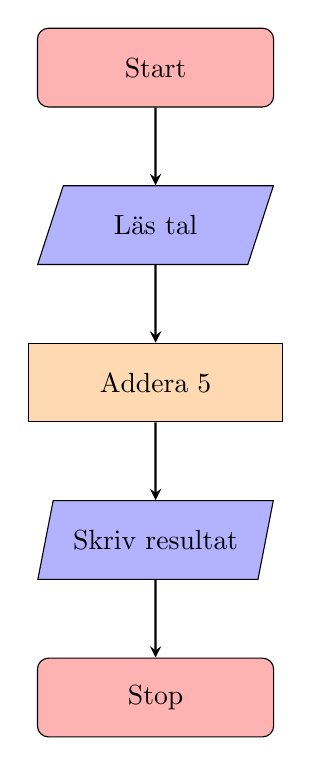
\begin{tikzpicture}[node distance=2cm]

\node (start) [startstop] {Start};
\node (input) [io, below of=start] {Läs tal};
\node (process) [process, below of=input] {Addera 5};
\node (output) [io, below of=process] {Skriv resultat};
\node (stop) [startstop, below of=output] {Stop};

\draw [arrow] (start) -- (input);
\draw [arrow] (input) -- (process);
\draw [arrow] (process) -- (output);
\draw [arrow] (output) -- (stop);

\end{tikzpicture}
\end{center}

För att följa ett flödesdiagram så börjar vi i start-rutan, och följer pilarna. 
Vid varje ny symbol så utför vi det som står där, exempelvis fråga användaren efter ett tal. 
Så småningom så kommer vi nå stop-symbolen och då är programmet slut. 
Flödesdiagram är till för att beskriva ett program, men behöver inte skrivas på ett
lika exakt sätt som pythonkod. 
Vi kan därför skriva saker som ''Läs tal'' och räkna med att den som läser
flödesdiagrammet förstår att när vi sen skriver ''Addera 5'' menar vi ''Addera 5 till talet och spara det nya värdet till tal''.
Hur formellt och noga man ska skriva sina flödesdiagram är delvis en smaksak. 
Målet är däremot att det ska vara tydligt hur det fungerar. Kanske tycker du inte det är självklart vad ''Addera 5'' innebär i flödesdiagrammet ovan. 

Vi kan också översätta vårat flödesdiagram till pythonkod:

\textbf{Motsvarande Python-kod:}
\begin{lstlisting}[language=Python]
# Läs ett tal från användaren
nummer = int(input("Ange ett tal: "))

# Lägg till 5
resultat = nummer + 5

# Skriv ut resultatet
print("Resultatet är:", resultat)
\end{lstlisting}

\pythonoutput{Exempel output}{
Ange ett tal: 10\\
Resultatet är: 15
}

Exempel: Beslutsstruktur
I många program måste beslut tas beroende på data. Beslutsstrukturer visas i flödesdiagram med en romb.

\textbf{Flödesdiagram:}
\begin{center}
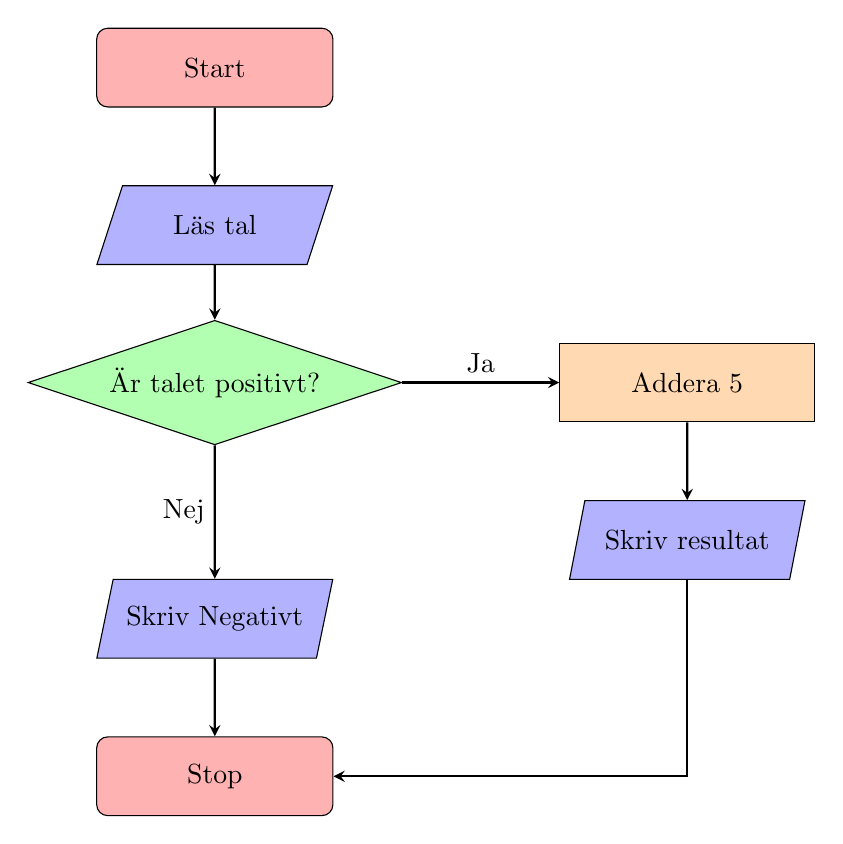
\begin{tikzpicture}[node distance=2cm]

\node (start) [startstop] {Start};
\node (input) [io, below of=start] {Läs tal};
\node (decision) [decision, below of=input] {Är talet positivt?};
\node (process) [process, right of=decision, xshift=4cm] {Addera 5};
\node (output1) [io, below of=process] {Skriv resultat};
\node (output2) [io, below of=decision, yshift=-1cm] {Skriv Negativt};
\node (stop) [startstop, below of=output2] {Stop};

\draw [arrow] (start) -- (input);
\draw [arrow] (input) -- (decision);
\draw [arrow] (decision.east) -- node[anchor=south] {Ja} (process.west);
\draw [arrow] (process) -- (output1);
\draw [arrow] (decision.south) -- node[anchor=east] {Nej} (output2.north);
\draw [arrow] (output1.south) |- (stop.east);
\draw [arrow] (output2) -- (stop);

\end{tikzpicture}
\end{center}

I programmet ser du romb eller diamantsymbolen som motsvarar en if-sats i programmeringskod. 
Det är den ända symbolen i flödesdiagram som det kan gå ut mer än en pil från. 
Notera också att pilarna som går ut från diamantsymbolen är markerade med Ja och Nej för att visa
vid vilka fall vi ska gå vilken väg. 
I detta fall så går vi på Ja-pilen om talet är positivt. Eller Nej pilen om talet inte är positivt. 
Det som står i en diamantsymbol är alltså alltid en ja-nej-fråga. 

\textbf{Motsvarande Python-kod:}
\begin{lstlisting}[language=Python]
# Läs ett tal från användaren
nummer = int(input("Ange ett tal: "))

if nummer > 0:
    # Om talet är positivt, addera 5
    resultat = nummer + 5
    print("Resultatet är:", resultat)
else:
    # Om talet är negativt, skriv "Negativt"
    print("Talet är negativt")
\end{lstlisting}

\pythonoutput{Exempel output 1}{
Ange ett tal: 3\\
Resultatet är: 8
}

\pythonoutput{Exempel output 2}{
Ange ett tal: -5\\
Talet är negativt
}

Om vi har ett program med en while-loop är det ända vi behöver göra
att dra en pil tillbaka till ett tidigare steg. 
En while-loop avbryts när ett villkor är falskt så vi kan använda
våran vanliga diamantsymbol. 
Genom att på detta sätt återanvända delar av ett flödesdiagram kan vi på samma
sätt som i programmeringskod beskriva mera komplicerade processer.

\begin{tabular*}{\linewidth}{@{\extracolsep{\fill}} p{0.55\linewidth} | p{0.45\linewidth}}
\textbf{Flödesdiagram:} & \textbf{Python-kod:} \\
\hline

% Flödesdiagram
\raisebox{-\totalheight}{%
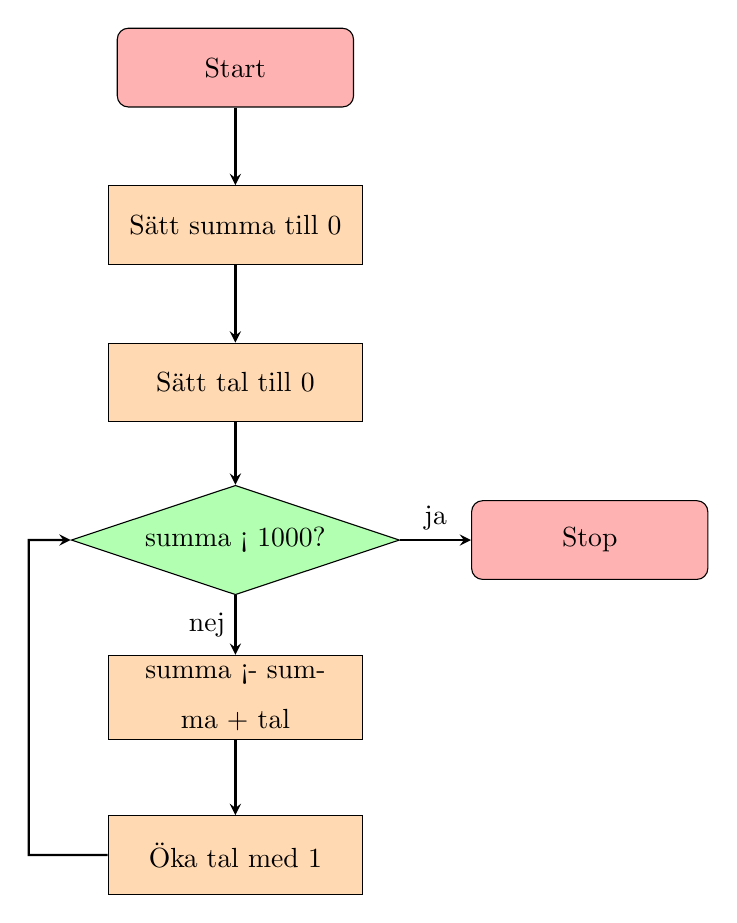
\begin{tikzpicture}[node distance=2cm]
\node (start) [startstop] {Start};
\node (summainit) [process, below of=start] {Sätt summa till 0};
\node (talinit) [process, below of=summainit] {Sätt tal till 0};
\node (decision) [decision, below of=talinit] {summa < 1000?};
\node (summera) [process, below of=decision] {summa <- summa + tal};
\node (ökatal) [process, below of=summera] {Öka tal med 1};
\node (stop) [startstop, right of=decision, xshift=2.5cm] {Stop};

\draw [arrow] (start) -- (summainit);
\draw [arrow] (summainit) -- (talinit);
\draw [arrow] (talinit) -- (decision);
\draw [arrow] (decision.east) -- node[anchor=south] {ja} (stop.west);
\draw [arrow] (decision.south) -- node[anchor=east] {nej} (summera);
\draw [arrow] (summera) -- (ökatal);
\draw [arrow] (ökatal.west) -- ++(-1,0) -- ++(0,4) -- (decision.west);

%\draw [arrow] (ökatal) -- (decision.west);

\end{tikzpicture}
}
&

% Python-kod
\raggedright
\begin{lstlisting}[caption={Summera positiva tal}, xleftmargin=1.5em]
# Räknar 1+2+3+4+5... så länge summan är mindre än 1000
summa = 0
tal = 1
while summa < 1000:
    summa = summa + tal

print("Summa 1+2+3+...+",tal,">1000")

\end{lstlisting}
\vspace{0.5em}
Räknar ut vilket tal vi behöver räkna till så att $1+2+3+\cdots+tal>1000$.
\\
\end{tabular*}
\observera{I detta flödesdiagram har vi varit lite mer noga med att beskriva variabler än i tidigare exempel. 
Det är som sagt inte en exakt vetenskap hur det ska beskrivas, men eftersom vi i programmet håller reda på både 
summan av alla tal, och vilket tal vi ligger på, kan det vara bra att vara lite extra tydlig. 
Notera också att vi skrivit \textbf{summa <- summa + tal} istället för \textbf{summa = summa + tal}. 
Det är vanligt att man använder en pil för att beskriva tilldelning till en variabel när man skriver flödesdiagram, eller psuedokod vilket vi tar upp i ett senare avsnitt
}


Sammanfattning:
Flödesdiagram är ett kraftfullt verktyg för att planera och analysera programlogik. Genom att översätta diagram till kod (och vice versa) kan du få en bättre förståelse för hur program fungerar.

\secToExRef{examples:flowchart}

\newpage
\section{Logiska uttryck och booleanska värden}
\label{section:boolean}
\subsection{Vad är ett logiskt uttryck?}
Ett logiskt uttryck är ett uttryck som antingen är \textbf{sant} (\texttt{True}) eller \textbf{falskt} (\texttt{False}). Logiska uttryck används ofta i beslutsfattande, till exempel i \texttt{if}-satser och loopar, för att avgöra om en viss kod ska köras.

\begin{lstlisting}[title=Exempel på logiska uttryck]
x = 5
y = 10
print(x < y)  # True
print(x == y) # False
\end{lstlisting}

I exemplet ovan är \texttt{x < y} sant eftersom \texttt{5} är mindre än \texttt{10}. Däremot är \texttt{x == y} falskt eftersom \texttt{5} inte är lika med \texttt{10}.

\begrepp{Boolean}{En datatyp i Python som kan vara \texttt{True} (sant) eller \texttt{False} (falskt). Den används i logiska uttryck.}

\subsection{Logiska operatorer}
Python har tre logiska operatorer: \texttt{and}, \texttt{or}, och \texttt{not}. Dessa används för att kombinera eller invertera logiska uttryck.

\subsubsection{\textbf{and}}
Operatorn \texttt{and} returnerar \texttt{True} om båda uttrycken är sanna.
\begin{lstlisting}[title=Exempel med \texttt{and}]
x = 5
y = 10
z = 15

print(x < y and y < z)  # True (båda villkoren är sanna)
print(x > y and y < z)  # False (det första villkoret är falskt)
\end{lstlisting}

\subsubsection{\textbf{or}}
Operatorn \texttt{or} returnerar \texttt{True} om minst ett av uttrycken är sant.
\begin{lstlisting}[title=Exempel med \texttt{or}]
x = 5
y = 10

print(x > y or x < y)   # True (det andra villkoret är sant)
print(x > y or y > 20)  # False (båda villkoren är falska)
\end{lstlisting}

\subsubsection{\textbf{not}}
Operatorn \texttt{not} inverterar värdet av ett logiskt uttryck.
\begin{lstlisting}[title=Exempel med \texttt{not}]
x = 5
y = 10

print(not x < y)  # False (inverterar värdet av "x < y", som är True)
\end{lstlisting}

\subsection{Praktiskt exempel: Kontrollera behörighet}
Här är ett exempel där logiska operatorer används för att avgöra om en person är behörig att rösta.
\begin{lstlisting}[title=Exempel med behörighetskontroll]
alder = int(input("Hur gammal är du? "))

if alder >= 18 and alder < 120:
    print("Du får rösta!")
else:
    print("Du är inte behörig att rösta.")
\end{lstlisting}

I detta program kontrolleras om åldern är 18 år eller äldre och mindre än 120.

\subsection{Övningar}
\begin{exercise}
Skriv ett program som frågar användaren efter ett nummer. Programmet ska skriva ut \texttt{True} om numret är mellan 10 och 20, annars \texttt{False}.
\end{exercise}

\begin{solution}
\begin{lstlisting}
nummer = int(input("Skriv in ett nummer: "))
print(nummer >= 10 and nummer <= 20)
\end{lstlisting}
\end{solution}

\begin{exercise}
Skriv ett program som frågar användaren efter två tal. Programmet ska skriva ut \texttt{True} om minst ett av talen är större än 50.
\end{exercise}

\begin{solution}
\begin{lstlisting}
tal1 = int(input("Skriv in det första talet: "))
tal2 = int(input("Skriv in det andra talet: "))
print(tal1 > 50 or tal2 > 50)
\end{lstlisting}
\end{solution}

\begin{exercise}
Skriv ett program som frågar användaren efter ett lösenord. Om lösenordet är \texttt{hemligt123} ska programmet skriva \texttt{Access granted}, annars \texttt{Access denied}.
\end{exercise}

\begin{solution}
\begin{lstlisting}
losenord = input("Skriv in ditt lösenord: ")

if losenord == "hemligt123":
    print("Access granted")
else:
    print("Access denied")
\end{lstlisting}
\end{solution}

\secToExRef{examples:boolean}

\newpage
\section{Matematik i Python: \texttt{math}-modulen och specialoperatorer}
\label{section:math}
Python har inbyggda verktyg för matematiska beräkningar. Förutom grundläggande operatorer som \texttt{+}, \texttt{-}, \texttt{*}, och \texttt{/} finns fler avancerade funktioner i \texttt{math}-modulen. Här ska vi även titta på specialoperatorerna \texttt{**}, \texttt{\%}, och \texttt{//}.

\subsection{\texttt{math}-modulen}
\texttt{math}-modulen är en inbyggd modul i Python som erbjuder en mängd matematiska funktioner och konstanter.

\subsubsection{Importera \texttt{math}-modulen}
För att använda modulen måste den importeras i din kod:
\begin{lstlisting}[title=Exempel: Importera \texttt{math}]
import math
\end{lstlisting}

Efter att du har importerat \texttt{math} kan du använda dess funktioner.

\subsubsection{Vanliga funktioner i \texttt{math}}
Här är några av de mest använda funktionerna i \texttt{math}:
\begin{lstlisting}[title=Exempel på \texttt{math}-funktioner]
import math

# Roten ur ett tal
print(math.sqrt(16))  # 4.0

# Upphöjning till en viss potens
print(math.pow(2, 3))  # 8.0

# Heltalsdel av en division
print(math.floor(7.8))  # 7
print(math.ceil(7.2))   # 8

# Värdet av pi och e
print(math.pi)  # 3.141592653589793
print(math.e)   # 2.718281828459045
\end{lstlisting}

\begrepp{Modul}{En modul är ett bibliotek av funktioner och variabler som kan importeras och användas i ett program.}

\subsection{Specialoperatorer}
Python har flera operatorer som är användbara för matematiska beräkningar utöver de grundläggande.

\subsubsection{\texttt{**} (Exponentiering)}
Operatorn \texttt{**} används för att upphöja ett tal till en viss potens.
\begin{lstlisting}[title=Exempel på \texttt{**}]
print(2 ** 3)  # 8 (2 upphöjt till 3)
print(5 ** 2)  # 25 (5 upphöjt till 2)
\end{lstlisting}

\subsubsection{\texttt{\%} (Modulus)}
Operatorn \texttt{\%} returnerar resten vid en division.
\begin{lstlisting}[title=Exempel på \texttt{\%}]
print(10 % 3)  # 1 (10 dividerat med 3 ger resten 1)
print(15 % 4)  # 3 (15 dividerat med 4 ger resten 3)
\end{lstlisting}

\begrepp{Modulus}{En operation som returnerar resten vid division av två tal.}

\subsubsection{\texttt{//} (Heltalsdivision)}
Operatorn \texttt{//} utför division och returnerar endast heltalsdelen av resultatet.
\begin{lstlisting}[title=Exempel på \texttt{//}]
print(10 // 3)  # 3 (heltalsdelen av 10 dividerat med 3)
print(15 // 4)  # 3 (heltalsdelen av 15 dividerat med 4)
\end{lstlisting}

\begrepp{Heltalsdivision}{En operation som returnerar heltalsdelen av en division, utan decimaler.}

\subsection{Praktiskt exempel: Beräkna cirkelns area}
Här använder vi \texttt{math}-modulen och en av specialoperatorerna för att beräkna en cirkels area.
\begin{lstlisting}[title=Beräkna cirkelns area]
import math

# Fråga användaren efter radien
radie = float(input("Ange radien: "))

# Beräkna arean
area = math.pi * (radie ** 2)
print("Cirkelns area är:", area)
\end{lstlisting}

\subsection{Övningar}
\begin{exercise}
Skriv ett program som använder \texttt{math.sqrt()} för att beräkna kvadratroten av ett tal som användaren anger.
\end{exercise}

\begin{solution}
\begin{lstlisting}
import math

# Fråga användaren efter ett tal
tal = float(input("Ange ett tal: "))

# Beräkna och visa kvadratroten
print("Kvadratroten av", tal, "är:", math.sqrt(tal))
\end{lstlisting}
\end{solution}

\begin{exercise}
Skriv ett program som använder \texttt{\%} för att avgöra om ett tal som användaren anger är jämnt eller udda.
\end{exercise}

\begin{solution}
\begin{lstlisting}
# Fråga användaren efter ett tal
tal = int(input("Ange ett tal: "))

# Kontrollera om talet är jämnt eller udda
if tal % 2 == 0:
    print("Talet är jämnt.")
else:
    print("Talet är udda.")
\end{lstlisting}
\end{solution}

\begin{exercise}
Skriv ett program som frågar användaren efter två tal och skriver ut resultatet av \texttt{//} och \texttt{\%}.
\end{exercise}

\begin{solution}
\begin{lstlisting}
# Fråga användaren efter två tal
tal1 = int(input("Ange det första talet: "))
tal2 = int(input("Ange det andra talet: "))

# Beräkna heltalsdivision och resten
print("Heltalsdivision:", tal1 // tal2)
print("Rest:", tal1 % tal2)
\end{lstlisting}
\end{solution}

\secToExRef{examples:math}



\chapter{Funktioner och datastrukturer}
\section{Listor i Python}
\label{section:lists}
Listor är en av de mest användbara datatyperna i Python. De används för att lagra flera värden i en och samma variabel. Till exempel kan en lista innehålla en samling av tal, strängar eller till och med andra listor.

\subsection{Skapa en lista}
En lista skapas genom att använda hakparenteser \texttt{[]} och separera elementen med kommatecken:
\begin{lstlisting}[title=Exempel: Skapa en lista]
# En lista med tal
tal = [1, 2, 3, 4, 5]

# En lista med text
djur = ["katt", "hund", "kanin"]

# En blandad lista
blandad = [1, "äpple", True]
\end{lstlisting}

\begrepp{Lista}{En lista är en samling av värden som kan lagras i en variabel.}
\begrepp{Element}{Ett värde i listan kallas för ett element}

\subsection{Åtkomst till element i en lista}
Varje element i en lista har ett index som börjar på \texttt{0} för det första elementet. Du kan komma åt ett element genom att ange dess index inom hakparenteser:
\begin{lstlisting}[title=Exempel: Åtkomst via index]
djur = ["katt", "hund", "kanin"]
print(djur[0])  # Skriv ut "katt"
print(djur[1])  # Skriv ut "hund"
\end{lstlisting}

\begrepp{Index}{Index är platsen på ett av listans värden. I python anges första elementet med index 0.}

\subsection{Modifiera en lista}
Du kan ändra värdet på ett element, lägga till nya element eller ta bort befintliga element.

\paragraph{Ändra värde:}
\begin{lstlisting}[title=Exempel: Ändra värde]
djur = ["katt", "hund", "kanin"]
djur[1] = "hamster"  # Ändra "hund" till "hamster"
print(djur)  # ["katt", "hamster", "kanin"]
\end{lstlisting}

\paragraph{Lägga till element:}
\begin{lstlisting}[title=Exempel: Lägga till element]
djur = ["katt", "hund"]
djur.append("kanin")  # Lägg till "kanin" sist i listan
print(djur)  # ["katt", "hund", "kanin"]
\end{lstlisting}

\paragraph{Ta bort element:}
\begin{lstlisting}[title=Exempel: Ta bort element]
djur = ["katt", "hund", "kanin"]
djur.remove("hund")  # Ta bort "hund"
print(djur)  # ["katt", "kanin"]
\end{lstlisting}

\subsection{Loopar genom en lista}
Det är vanligt att använda loopar för att bearbeta alla element i en lista.
Vi kommer i nästa avsnitt se att man vanligen gör detta med en for-loop. 
Vi använder i detta exempel en while-loop eftersom det är vad vi sett hittills. 
\begin{lstlisting}[title=Exempel: For-loop med en lista]
djur = ["katt", "hund", "kanin"]
i = 0
while i<djur.len(): #Kör loopen tills i når slutet på listan
  print(djur[i])
  i = i + 1

# Skriver ut:
# katt
# hund
# kanin
\end{lstlisting}

Notera att vi kör programmet till variabeln \textbf{i} har ett värde som är ett mindre än listans längd.
Eftersom vi börjar räkna på 0 får vi ändå med alla tal. 
Inuti loopen använder vi våran variabel \textbf{i} för att skriva ut
ett element i listan i taget. 

\observera{Vi använder vanligen en variabel med namnet \textbf{i} för att beskriva ett index}

\subsection{Index out of bounds}
Ett vanligt fel när man jobbar med listor är ett ''Index out of bounds''-error.
Det betyder att vi har försökt hämta ett element (Ett värde i listan) som ligger utanför listan.
Om vi i en lista med 4 element försöker hämta det 5 elementet får vi det felet.
\begin{lstlisting}[title=Index out of bounds error]
tal = [1,2,3,4]
print(tal[5])
\end{lstlisting}

\begrepp{Index out of bounds-error}{En typ av fel vi får när vi försöker hämta ett element från en lista som ligger utanför listan.}

\subsection{Vanliga metoder för listor}
Python erbjuder flera metoder för att arbeta med listor:
\begin{itemize}
    \item \texttt{append()}: Lägg till ett element i slutet.
    \item \texttt{remove()}: Ta bort ett specifikt element.
    \item \texttt{pop()}: Ta bort och returnera det sista elementet (eller ett specifikt index).
    \item \texttt{sort()}: Sortera listan.
    \item \texttt{len()}: Returnera antalet element i listan.
\end{itemize}
\begin{lstlisting}[title=Exempel: Använda lista-metoder]
djur = ["kanin", "hund", "katt"]
djur.sort()  # Sortera listan
print(djur)  # ["hund", "kanin", "katt"]
\end{lstlisting}

\subsection{Övningar}
\begin{exercise}
Skapa en lista med namnen på tre frukter och skriv ut dem en och en med en loop.
\end{exercise}
\begin{solution}
\begin{lstlisting}
frukter = ["äpple", "banan", "apelsin"]
for frukt in frukter:
    print(frukt)
\end{lstlisting}
\end{solution}

\begin{exercise}
Skapa en lista med siffrorna 1 till 5. Lägg till talet 6 och skriv sedan ut hela listan.
\end{exercise}
\begin{solution}
\begin{lstlisting}
tal = [1, 2, 3, 4, 5]
tal.append(6)
print(tal)  # [1, 2, 3, 4, 5, 6]
\end{lstlisting}
\end{solution}

\begin{exercise}
Skapa en lista med talen 10, 20 och 30. Använd \texttt{len()} för att skriva ut antalet element i listan.
\end{exercise}
\begin{solution}
\begin{lstlisting}
tal = [10, 20, 30]
print(len(tal))  # 3
\end{lstlisting}
\end{solution}

\secToExRef{examples:lists}

\newpage
\section{For-loop (Upprepa saker med Python)}
\label{section:for}

En \texttt{for}-loop används när vi vill upprepa något för varje sak i en lista, varje bokstav i en text, eller över en rad nummer. Tanken är enkel: loopen går igenom varje sak i listan, en i taget, och gör något med den.

\subsection{Hur fungerar en for-loop?}

En \texttt{for}-loop i Python ser ut så här:

\begin{lstlisting}[title=Syntax för for-loop]
for variabel in lista:
    # Gör något med variabeln
\end{lstlisting}

Vad händer steg för steg?\\

1. \textbf{Variabeln} är ett namn vi väljer. Den kommer att innehålla en sak från listan i taget.\\
2. \textbf{Listan} är det vi vill gå igenom, t.ex. en samling siffror eller bokstäver.\\
3. Loopen tar varje sak i listan och lagrar den i variabeln. Sedan kör den koden inuti loopen.\\

Exempel: Skriv ut siffror i en lista\\

Här är ett enkelt exempel där vi har en lista med siffror:

\begin{lstlisting}[title=Exempel: Skriv ut siffror]
tal_lista = [1, 2, 3, 4, 5]

for tal in tal_lista:
    print(tal)
\end{lstlisting}

Vad händer när programmet körs?

1. Första gången i loopen är \texttt{tal = 1}. Koden \texttt{print(tal)} körs och skriver ut 1.\\
2. Sedan hoppar loopen till nästa tal i listan, \texttt{tal = 2}, och skriver ut 2.\\
3. Detta fortsätter för alla tal i listan.\\

Resultatet blir:

\pythonoutput{Exempel: Output}{
1 \\
2 \\
3 \\
4 \\
5
}

\observera{Det är viktigt att koden inuti loopen är indenterad (indragen), annars får du fel. Python använder indrag för att veta vad som hör till loopen.}

\subsection{Ett tydligare exempel: Steg för steg}

Låt oss se ett ännu tydligare exempel. Här använder vi en lista med namn:

\begin{lstlisting}[title=Exempel: Skriv ut namn]
namn_lista = ["Anna", "Björn", "Cecilia"]

for namn in namn_lista:
    print("Hej, " + namn + "!")
\end{lstlisting}

Vad händer när programmet körs?

1. \textbf{Första varvet}: Variabeln \texttt{namn} blir \texttt{''Anna''}. Programmet skriver ut \texttt{"Hej, Anna!"}.\\
2. \textbf{Andra varvet}: Variabeln \texttt{namn} blir \texttt{''Björn''}. Programmet skriver ut \texttt{"Hej, Björn!"}.\\
3. \textbf{Tredje varvet}: Variabeln \texttt{namn} blir \texttt{''Cecilia''}. Programmet skriver ut \texttt{"Hej, Cecilia!"}.\\

Outputen blir:

\pythonoutput{Exempel: Output}{
Hej, Anna! \\
Hej, Björn! \\
Hej, Cecilia!
}


\subsection{For-loop med \texttt{range()}}
Vi kan också använda \texttt{range()} för att skapa en serie siffror automatiskt. Till exempel kan vi skriva ut talen från 1 till 5 utan att skapa en lista först:

\begin{lstlisting}[title=Exempel: range()]
for tal in range(1, 6):
    print(tal)
\end{lstlisting}

Här skapar \texttt{range(1, 6)} siffrorna 1 till 5 (men inte 6). Resultatet blir detsamma som med listan ovan.

\textbf{Steg i \texttt{range()}}\\
Du kan lägga till ett steg i \texttt{range()} för att hoppa över tal. Till exempel:
\begin{lstlisting}
for tal in range(2, 11, 2):
    print(tal)
\end{lstlisting}
Här hoppar \texttt{range()} två steg åt gången och skriver ut 2, 4, 6, 8, 10.


\subsection{For-loop med text}
En sträng i Python kan behandlas som en lista av bokstäver. Vi kan använda en \texttt{for}-loop för att skriva ut varje bokstav i en sträng:

\begin{lstlisting}[title=Exempel: Loopa över en sträng]
text = "Python"

for bokstav in text:
    print(bokstav)
\end{lstlisting}

Outputen blir:
\pythonoutput{Exempel: Output}{
P \\
y \\
t \\
h \\
o \\
n
}



\subsection{Övningar}
\begin{exercise}
Skriv ett program som skriver ut alla siffror från 1 till 10, en per rad.
\end{exercise}
\begin{solution}
\begin{lstlisting}
for tal in range(1, 11):
    print(tal)
\end{lstlisting}
\end{solution}

\begin{exercise}
Skriv ett program som skriver ut alla multiplar av 3 mellan 1 och 30.
\end{exercise}
\begin{solution}
\begin{lstlisting}
for tal in range(3, 31, 3):
    print(tal)
\end{lstlisting}
\end{solution}

\begin{exercise}
Skriv ett program som skriver ut varje bokstav i strängen ''Programmering'' på en ny rad.
\end{exercise}
\begin{solution}
\begin{lstlisting}
text = "Programmering"
for bokstav in text:
    print(bokstav)
\end{lstlisting}
\end{solution}

\secToExRef{examples:for}

\newpage
\section{Dictionary: En samling av nyckel-värde-par}
\label{section:dictionary}
En \textbf{dictionary} (eller ''ordbok'') i Python är en datastruktur som används för att lagra data i form av nyckel-värde-par. Detta innebär att varje värde i en dictionary är kopplat till en unik nyckel, som används för att referera till värdet. Detta gör dictionaries särskilt användbara när vi behöver hantera data som har en logisk koppling, till exempel namn och telefonnummer eller ord och deras definitioner.

\subsection{Skapa en dictionary}
En dictionary skapas genom att använda klamrar \texttt{\{\}} och separera nycklar och värden med kolon (\texttt{:}). Här är ett exempel:

\begin{lstlisting}[title=Skapa en dictionary]
# Skapa en dictionary med information om en person
person = {
    "namn": "Alice",
    "ålder": 25,
    "stad": "Stockholm"
}
\end{lstlisting}

\subsection{Åtkomst till värden}
För att hämta ett värde från en dictionary använder vi nyckeln inom hakparenteser \texttt{[]}:

\begin{lstlisting}[title=Hämta värden från en dictionary]
# Hämta värdet för nyckeln "namn"
print(person["namn"])  # Output: Alice
\end{lstlisting}

Om vi försöker använda en nyckel som inte finns i dictionaryn, kommer Python att generera ett \texttt{KeyError}. För att undvika detta kan vi använda metoden \texttt{get()}, som låter oss ange ett standardvärde:

\begin{lstlisting}[title=Använda get-metoden]
# Försök hämta en nyckel som inte finns
print(person.get("jobb", "Okänd"))  # Output: Okänd
\end{lstlisting}

\subsection{Lägga till och ändra värden}
Vi kan lägga till nya nyckel-värde-par eller ändra existerande värden:

\begin{lstlisting}[title=Lägga till och ändra värden]
# Lägg till en ny nyckel "jobb"
person["jobb"] = "Programmerare"

# Ändra värdet för nyckeln "stad"
person["stad"] = "Göteborg"

print(person)
\end{lstlisting}

\subsection{Ta bort värden}
Vi kan använda pop() för att ta bort ett nyckel-värde-par:

\begin{lstlisting}[title=Ta bort värden från en dictionary]
# Ta bort nyckeln "ålder"
person.pop("ålder")

print(person)
\end{lstlisting}

\subsection{Loopa genom en dictionary}
Vi kan loopa igenom en dictionary för att få åtkomst till dess nycklar och värden:

\begin{lstlisting}[title=Loop genom en dictionary]
# Loopa genom nycklar och värden
for nyckel, värde in person.items():
    print(f"{nyckel}: {värde}")
\end{lstlisting}

\subsection{Exempel på användning}
Här är ett exempel på hur dictionaries kan användas för att lagra och analysera data:

\begin{lstlisting}[title=Exempel: Räkna antalet bokstäver i en text]
# Räkna antalet förekomster av varje bokstav
text = "programmering"
bokstavsfrekvens = {}

for bokstav in text:
    bokstavsfrekvens[bokstav] = bokstavsfrekvens.get(bokstav, 0) + 1

print(bokstavsfrekvens)
\end{lstlisting}

\pythonoutput{Output}{
\texttt{\{}'p': 1, 'r': 3, 'o': 1, 'g': 2, 'a': 1, 'm': 2, 'e': 1, 'i': 1, 'n': 1\texttt{\}}
}

\subsection{Övningar}
\begin{exercise}
Skapa en dictionary som innehåller tre städer och deras befolkning. Skriv ut befolkningen för en av städerna.
\end{exercise}
\begin{solution}
\begin{lstlisting}
# Skapa en dictionary med städer och befolkning
stad_befolkning = {
    "Stockholm": 975551,
    "Göteborg": 583056,
    "Malmö": 347949
}

# Skriv ut befolkningen för en stad
print("Befolkning i Stockholm:", stad_befolkning["Stockholm"])
\end{lstlisting}
Output:
\pythonoutput{}{
Befolkning i Stockholm: 975551
}
\end{solution}

\begin{exercise}
Skriv ett program som använder en dictionary för att lagra elevbetyg. Programmet ska kunna lägga till nya elever och deras betyg samt visa alla sparade betyg.
\end{exercise}
\begin{solution}
\begin{lstlisting}
# Skapa en tom dictionary för elevbetyg
elev_betyg = {}

# Lägg till nya elever och deras betyg
elev_betyg["Anna"] = "A"
elev_betyg["Björn"] = "B"
elev_betyg["Cecilia"] = "C"

# Visa alla elever och deras betyg
print("Elevbetyg:")
for elev, betyg i elev_betyg.items():
    print(f"{elev}: {betyg}")
\end{lstlisting}
Output:
\pythonoutput{}{
Elevbetyg: \\
Anna: A \\
Björn: B \\
Cecilia: C
}
\end{solution}
\begin{exercise}
Skapa ett program som räknar hur många gånger varje bokstav förekommer i en given mening. 
Implementera detta genom att använda en \texttt{for}-loop och metoden \texttt{get()}.

\end{exercise}
\begin{solution}
\begin{lstlisting}
# Mening att analysera
mening = "Detta är en enkel mening"

# Skapa en tom dictionary för att räkna bokstäver
bokstav_räknare = {}

# Gå igenom varje bokstav i den rensade meningen
for bokstav in rensad_mening:
    # Använd get() för att öka antalet eller sätta det till 1 om bokstaven är ny
    bokstav_räknare[bokstav] = bokstav_räknare.get(bokstav, 0) + 1

# Visa resultatet
print("Antal bokstäver:")
for bokstav, antal in bokstav_räknare.items():
    print(f"{bokstav}: {antal}")
\end{lstlisting}
Output:
\pythonoutput{}{
Antal bokstäver: \\
d: 1 \\
e: 7 \\
t: 4 \\
a: 2 \\
ä: 1 \\
n: 4 \\
k: 1 \\
l: 1 \\
m: 1 \\
g: 1
}
\end{solution}

\secToExRef{examples:dictionary}

\newpage
\section{Funktioner: Strukturera och Återanvänd Kod}
\label{section:functions}

Funktioner är en grundläggande del av programmering. De låter oss strukturera kod genom att dela upp den i mindre, hanterbara delar. Funktioner kan också återanvändas, vilket gör vårt arbete effektivare och vår kod lättare att förstå och underhålla.

\subsection{Vad är en funktion?}
En funktion är en bit kod som utför en specifik uppgift. 
Vi definierar funktioner med nyckelordet \texttt{def} och ett namn, följt av eventuella parametrar inom parentes. 
Funktionen kan köras genom att vi anropar dess namn.

\begin{lstlisting}[title=En enkel funktion]
def hälsa():
    print("Hej! Välkommen till Python.")
    
hälsa()  # Anropa funktionen
\end{lstlisting}

\subsection{Parametrar och argument}
Vi kan ge funktioner indata genom att använda parametrar. När vi anropar funktionen skickar vi värden, som kallas argument, till parametrarna.

\begin{lstlisting}[title=Funktion med parametrar]
def hälsa(namn):
    print(f"Hej, {namn}! Välkommen till Python.")
    
hälsa("Alice")  # Output: Hej, Alice! Välkommen till Python.
\end{lstlisting}

\begrepp{Parameter}{En parameter är en plats för indata i en funktions definition.}
\begrepp{Argument}{Ett argument är det faktiska värde vi skickar till en funktions parameter.}

\subsection{Returvärden}
En funktion kan också ge tillbaka ett värde till det ställe där den anropas. Detta görs med nyckelordet \texttt{return}.

\begin{lstlisting}[title=Funktion med returvärde]
def addera(a, b):
    return a + b
    
resultat = addera(5, 7)
print(resultat)  # Output: 12
\end{lstlisting}

\begrepp{Returvärde}{Ett returvärde är det värde som en funktion skickar tillbaka till anropsplatsen med hjälp av \texttt{return}.}

\subsection{Main-funktionen}
I större program är det vanligt att använda en \texttt{main}-funktion för att tydligt visa var programmet börjar. Här är ett exempel:

\begin{lstlisting}[title=Ett program med en main-funktion]
def hälsa():
    print("Hej! Välkommen till Python.")
    
def main():
    hälsa()

if __name__ == "__main__":
    main()
\end{lstlisting}

När vi använder \texttt{if \_\_name\_\_ == "\_\_main\_\_"}, ser Python till att bara köra \texttt{main()} om programmet körs direkt, inte om det importeras i ett annat program.

\begrepp{Main-funktion}{En \texttt{main}-funktion fungerar som programmets startpunkt, vilket gör koden tydligare och mer strukturerad.}

\subsection{Namespace: Variabler i funktioner}
Varje funktion har sitt eget \textbf{namespace}, vilket innebär att variabler definierade i funktionen inte påverkar eller är kända utanför den. Här är ett exempel:

\begin{lstlisting}[title=Namespace och variabler]
def ändra_värde():
    x = 10  # Lokal variabel
    print(f"Inne i funktionen: {x}")
    
x = 5  # Global variabel
ändra_värde()
print(f"Utanför funktionen: {x}")
\end{lstlisting}

Output:
\begin{verbatim}
Inne i funktionen: 10
Utanför funktionen: 5
\end{verbatim}

I detta exempel är variabeln \texttt{x} inne i funktionen skild från variabeln \texttt{x} utanför. Detta förhindrar att funktioner oavsiktligt ändrar värden i resten av programmet.

\begrepp{Namespace}{Ett namespace är ett område där variabler och deras värden lagras. En funktions namespace är separat från resten av programmet.}

\subsection{Övningar}
\begin{exercise}
Skriv en funktion \texttt{dubbla()} som tar ett tal som parameter och returnerar dess dubbla värde.
\end{exercise}

\begin{exercise}
Skapa ett program med en \texttt{main}-funktion som anropar en funktion \texttt{hälsa(namn)} och skriver ut en personlig hälsning.
\end{exercise}

\begin{exercise}
Experimentera med namespace genom att skapa en funktion som definierar och ändrar en variabel. Kontrollera om förändringen påverkar en variabel med samma namn utanför funktionen.
\end{exercise}

\secToExRef{examples:functions}

\newpage

\chapter{Algoritmer}
\label{chapter:2}
\section*{Introduktion till algoritmer}
Algoritmer är grunden för all programmering. En algoritm är en serie steg som beskriver hur ett problem ska lösas. Genom att följa dessa steg kan vi skriva program som automatiserar beräkningar, sorterar data, söker efter information och mycket mer.

I detta kapitel kommer vi att utforska enkla och användbara algoritmer. Vi börjar med sorteringsalgoritmer, som hjälper oss att arrangera data i en viss ordning. Dessa algoritmer är inte bara praktiska, utan de lär oss också viktiga koncept som loopar, jämförelser och effektivitet.

Att förstå algoritmer handlar inte bara om att skriva kod, utan också om att tänka logiskt och lösa problem steg för steg. Oavsett om du programmerar ett spel, analyserar data eller skapar en hemsida, är algoritmer en central del av programmeringen.

\section{Bubble Sort}
\label{section:bubblesort}

\subsection*{Vad är Bubble Sort?}
Bubble Sort är en enkel sorteringsalgoritm som fungerar genom att jämföra två intilliggande element i en lista och byta plats på dem om de är i fel ordning. Den upprepar detta tills hela listan är sorterad. Namnet "Bubble Sort" kommer från att det största (eller minsta) elementet "bubblar" upp till sin rätta plats i varje iteration.

\subsection*{Hur fungerar Bubble Sort?}
Algoritmen går igenom listan flera gånger:
\begin{itemize}
    \item Jämför två intilliggande element.
    \item Om de är i fel ordning, byt plats på dem.
    \item Fortsätt jämföra nästa par tills slutet av listan är nådd.
    \item Upprepa detta tills hela listan är sorterad.
\end{itemize}

\subsection*{Kodexempel}
Här är en implementation av Bubble Sort i Python:
\begin{lstlisting}[title=Bubble Sort i Python]
def bubble_sort(lista):
    n = len(lista)
    for i in range(n):
        for j in range(0, n-i-1):
            if lista[j] > lista[j+1]:
                # Byt plats
                lista[j], lista[j+1] = lista[j+1], lista[j]

# Exempel
data = [64, 34, 25, 12, 22, 11, 90]
bubble_sort(data)
print("Sorterad lista:", data)
\end{lstlisting}

\subsection*{Förklaring av koden}
\begin{enumerate}
    \item \texttt{for i in range(n)}: Loopar genom listan flera gånger.
    \item \texttt{for j in range(0, n-i-1)}: Ser till att algoritmen inte jämför element som redan är sorterade.
    \item \texttt{if lista[j] > lista[j+1]}: Kontrollerar om elementen är i fel ordning.
    \item \texttt{lista[j], lista[j+1] = lista[j+1], lista[j]}: Byter plats på elementen.
\end{enumerate}

\subsection*{Visualisering}
Bubble Sort kan visualiseras som att sorteringen sker steg för steg, där varje större element "flyter upp" till toppen.

\subsection*{Övning}
\begin{exercise}
Implementera Bubble Sort för en lista som innehåller följande värden: \texttt{[10, 8, 2, 7, 1, 3]} och skriv ut den sorterade listan.
\end{exercise}
\begin{solution}
\begin{lstlisting}
data = [10, 8, 2, 7, 1, 3]
bubble_sort(data)
print("Sorterad lista:", data)
\end{lstlisting}
Output: \texttt{[1, 2, 3, 7, 8, 10]}
\end{solution}

\subsection*{Nackdelar med Bubble Sort}
Bubble Sort är enkel att förstå, men den är inte särskilt effektiv för långa listor eftersom den har en tidskomplexitet på \(O(n^2)\). Detta innebär att tiden det tar att sortera listan ökar kvadratiskt med dess storlek. För större datamängder är mer avancerade algoritmer, som Quick Sort eller Merge Sort, bättre val.

\secToExRef{examples:bubblesort}

\newpage
\section{Sökning}
\label{section:search}
När vi arbetar med data är det vanligt att vi behöver hitta ett specifikt värde i en samling, som en lista. Det finns olika sätt att göra detta, beroende på hur data är organiserad. Två grundläggande sökalgoritmer är \textbf{linjär sökning} och \textbf{binär sökning}.

\subsection{Linjär sökning}
Linjär sökning är den enklaste sökalgoritmen. Den går igenom varje element i listan, ett i taget, tills det hittar det sökta värdet eller når slutet av listan.

\begin{itemize}
    \item Fördel: Fungerar på både sorterade och osorterade listor.
    \item Nackdel: Kan vara långsam för långa listor eftersom varje element måste kontrolleras.
\end{itemize}

\subsubsection*{Kodexempel}
Här är ett exempel på linjär sökning i Python:
\begin{lstlisting}[title=Linjär sökning]
def linjar_sokning(lista, mål):
    for index, värde i enumerate(lista):
        if värde == mål:
            return index  # Returnerar positionen
    return -1  # Returnerar -1 om värdet inte finns

# Exempel
data = [10, 20, 30, 40, 50]
print(linjar_sokning(data, 30))  # Output: 2
\end{lstlisting}

\subsection{Binär sökning}
Binär sökning är en mer effektiv algoritm för att hitta ett värde i en sorterad lista. Algoritmen delar listan på mitten och avgör om det sökta värdet är mindre eller större än mittpunkten. Därefter upprepas processen på den relevanta halvan av listan.

\begin{itemize}
    \item Fördel: Mycket snabbare än linjär sökning för stora listor.
    \item Nackdel: Kräver att listan är sorterad.
\end{itemize}

\subsubsection*{Hur fungerar binär sökning?}
\begin{enumerate}
    \item Dela listan på mitten.
    \item Kontrollera mittpunkten:
        \begin{itemize}
            \item Om värdet är det sökta, är vi klara.
            \item Om värdet är mindre än det sökta, leta i den högra halvan.
            \item Om värdet är större, leta i den vänstra halvan.
        \end{itemize}
    \item Upprepa tills värdet hittas eller listan är tom.
\end{enumerate}

\subsubsection*{Kodexempel}
Här är ett exempel på binär sökning i Python:
\begin{lstlisting}[title=Binär sökning]
def binar_sokning(lista, mål):
    vänster, höger = 0, len(lista) - 1
    while vänster <= höger:
        mitten = (vänster + höger) // 2
        if lista[mitten] == mål:
            return mitten
        elif lista[mitten] < mål:
            vänster = mitten + 1
        else:
            höger = mitten - 1
    return -1  # Returnerar -1 om värdet inte finns

# Exempel
data = [10, 20, 30, 40, 50]
print(binar_sokning(data, 30))  # Output: 2
\end{lstlisting}

\subsection{Jämförelse mellan linjär och binär sökning}
\begin{table}[h!]
\centering
\begin{tabular}{|l|l|l|}
\hline
\textbf{Egenskap} & \textbf{Linjär sökning} & \textbf{Binär sökning} \\ \hline
Krav på sortering  & Nej                      & Ja                     \\ \hline
Effektivitet       & Långsam för långa listor & Snabb för långa listor \\ \hline
Komplexitet        & \(O(n)\)                & \(O(\log n)\)          \\ \hline
\end{tabular}
\caption{Jämförelse mellan linjär och binär sökning.}
\end{table}

\subsection{Övning}
\begin{exercise}
Skriv en Python-funktion som implementerar linjär sökning och använd den för att hitta värdet 25 i listan \texttt{[5, 15, 25, 35, 45]}.
\end{exercise}

\begin{exercise}
Använd kodexemplet för binär sökning för att hitta värdet 50 i listan \texttt{[10, 20, 30, 40, 50]}.
\end{exercise}

\secToExRef{examples:search}

\newpage
\section{Pseudokod}
\label{section:psuedocode}
Pseudokod är en metod för att beskriva algoritmer på ett sätt som är lätt att läsa och förstå, utan att behöva använda den exakta syntaxen i ett programmeringsspråk. Det fungerar som en mellanliggande representation som hjälper oss att planera och strukturera vår kod innan vi implementerar den.

\subsection{Varför använda pseudokod?}
Pseudokod är användbart eftersom det:
\begin{itemize}
    \item Hjälper till att fokusera på logiken i en algoritm, utan att fastna i språkspecifik syntax.
    \item Är enkelt att läsa och förstå, även för personer som inte är programmerare.
    \item Underlättar planeringen av mer komplexa program.
\end{itemize}

\subsection{Hur skriver man pseudokod?}
Det finns inga fasta regler för pseudokod, men här är några riktlinjer:
\begin{itemize}
    \item Använd beskrivande namn för variabler och steg.
    \item Håll det kortfattat och tydligt.
    \item Strukturera koden med indragningar för att visa block som hör ihop.
    \item Använd enkla termer som "LOOP", "IF", och "ELSE".
\end{itemize}

\subsection{Exempel: Summera en lista}
Låt oss skriva pseudokod för att summera alla värden i en lista.

\textbf{Pseudokod:}
\begin{verbatim}
START
SET summa TO 0
FOR varje element i listan:
    ADD element TO summa
END FOR
PRINT summa
END
\end{verbatim}

\textbf{Python-implementation:}
\begin{lstlisting}[title=Summera en lista]
lista = [1, 2, 3, 4, 5]
summa = 0
for element in lista:
    summa += element
print(summa)  # Output: 15
\end{lstlisting}

\subsection{Exempel: Hitta det största talet i en lista}
Här är ett exempel på pseudokod för att hitta det största talet i en lista.

\textbf{Pseudokod:}
\begin{verbatim}
START
SET största TO första elementet i listan
FOR varje element i listan:
    IF element > största:
        SET största TO element
    END IF
END FOR
PRINT största
END
\end{verbatim}

\textbf{Python-implementation:}
\begin{lstlisting}[title=Hitta största talet i en lista]
lista = [10, 20, 5, 30, 15]
största = lista[0]
for element in lista:
    if element > största:
        största = element
print(största)  # Output: 30
\end{lstlisting}

\subsection{Övningar}
\begin{exercise}
Skriv pseudokod för att räkna hur många jämna tal som finns i en lista.
\end{exercise}

\begin{exercise}
Implementera följande pseudokod i Python: \\
\texttt{START \\
SET antal TO 0 \\
FOR varje element i listan: \\
    IF element är större än 10: \\
        ADD 1 TO antal \\
    END IF \\
END FOR \\
PRINT antal \\
END}
\end{exercise}

\begin{rconceptbox}{Pseudokod}{Ett sätt att beskriva algoritmer med ord och strukturer som påminner om kod, men utan att följa strikt syntax.}
\end{rconceptbox}

\secToExRef{examples:psuedocode}

\newpage
\section{Rekursion}
\label{section:recursion}
Rekursion är en viktig programmeringsteknik där en funktion anropar sig själv för att lösa ett problem. Det kan vara användbart när ett problem kan delas upp i mindre, likartade delproblem.

\subsection{Hur fungerar rekursion?}
En rekursiv funktion måste alltid ha:
\begin{enumerate}
    \item \textbf{Basfall:} En villkorssats som avslutar rekursionen när ett visst kriterium uppfylls.
    \item \textbf{Rekursivt fall:} Ett anrop till sig själv, med ett argument som gradvis närmar sig basfallet.
\end{enumerate}

\subsection{Exempel: Faktorial}
Faktorial av ett heltal \( n \) definieras som:
\[
n! = n \times (n-1) \times (n-2) \times \dots \times 1
\]
Faktorial av 0 är definierat som 1 (\( 0! = 1 \)).

Med rekursion kan vi definiera detta som:
\[
n! = 
\begin{cases} 
1 & \text{om } n = 0 \\
n \times (n-1)! & \text{om } n > 0
\end{cases}
\]

\subsubsection*{Kodexempel}
\begin{lstlisting}[title=Rekursiv faktorialfunktion]
def faktorial(n):
    if n == 0:  # Basfall
        return 1
    else:       # Rekursivt fall
        return n * faktorial(n - 1)

# Exempel
print(faktorial(5))  # Output: 120
\end{lstlisting}

\begin{rconceptbox}{Rekursiv funktion}{En funktion som anropar sig själv. Den använder basfall för att avsluta anropen.}
\end{rconceptbox}

\subsection{Exempel: Rekursiv binär sökning}
Binär sökning kan också implementeras rekursivt. Istället för att använda en loop delar den rekursiva versionen listan i mindre delar tills det sökta värdet hittas eller listan är tom.

\subsubsection*{Kodexempel}
\begin{lstlisting}[title=Rekursiv binär sökning]
def rekursiv_binar_sokning(lista, mål, vänster, höger):
    if vänster > höger:  # Basfall: Målet finns inte
        return -1
    mitten = (vänster + höger) // 2
    if lista[mitten] == mål:  # Basfall: Målet hittas
        return mitten
    elif lista[mitten] < mål:
        return rekursiv_binar_sokning(lista, mål, mitten + 1, höger)
    else:
        return rekursiv_binar_sokning(lista, mål, vänster, mitten - 1)

# Exempel
data = [10, 20, 30, 40, 50]
print(rekursiv_binar_sokning(data, 30, 0, len(data) - 1))  # Output: 2
\end{lstlisting}

\subsection{Rekursion jämfört med iteration}
Rekursion och iteration (loopar) kan ofta lösa samma problem. Här är några skillnader:
\begin{itemize}
    \item \textbf{Rekursion:} Kan vara enklare och mer intuitiv för vissa problem, t.ex. träd eller grafproblem.
    \item \textbf{Iteration:} Mer minneseffektiv, eftersom rekursion kräver att varje anrop lagras på ett stackminne.
\end{itemize}

\begin{table}[h!]
\centering
\begin{tabular}{|l|l|}
\hline
\textbf{Fördelar med rekursion} & \textbf{Nackdelar med rekursion} \\ \hline
Intuitiv för vissa problem      & Kräver mer minne                 \\ \hline
Kortare kod i vissa fall        & Risk för stack overflow          \\ \hline
\end{tabular}
\caption{Jämförelse av rekursionens fördelar och nackdelar.}
\end{table}

\subsection{Övningar}
\begin{exercise}
Skriv en rekursiv funktion som beräknar summan av alla heltal från 1 till \( n \).
\end{exercise}

\begin{exercise}
Implementera binär sökning rekursivt och använd den för att hitta värdet 45 i listan \texttt{[5, 15, 25, 35, 45, 55]}.
\end{exercise}

\secToExRef{examples:recursion}

\newpage
%\chapter{Spelprogrammering}
\chapter{Lösningsförslag}
\printsolutions[headings=false]


\appendix
\chapter{Exempelkod}
Här finns exempelkod från varje kapitel. Syftet är att du ska kunna kolla på programmen för att förstå hur programmering kan användas. 

\section{Kodexempel: Print}
\label{examples:print}
\exToSecRef{section:print}
\subsection*{Grundläggande exempel}

\begin{lstlisting}[title=Exempel 1: Skriv ut en enkel text]
print("Hej, världen!")
\end{lstlisting}

\begin{lstlisting}[title=Exempel 2: Enkelcitat för text]
print('Python är roligt!')
\end{lstlisting}

\begin{lstlisting}[title=Exempel 3: Kombinera citattecken]
print("Han sa: 'Hej där!'")
\end{lstlisting}

\subsection*{Matematiska operationer}

\begin{lstlisting}[title=Exempel 4: Addition]
print(2 + 3)  # Output: 5
\end{lstlisting}

\begin{lstlisting}[title=Exempel 5: Subtraktion]
print(10 - 4)  # Output: 6
\end{lstlisting}

\begin{lstlisting}[title=Exempel 6: Multiplikation]
print(7 * 2)  # Output: 14
\end{lstlisting}

\begin{lstlisting}[title=Exempel 7: Division]
print(9 / 3)  # Output: 3.0
\end{lstlisting}

\begin{lstlisting}[title=Exempel 8: Parenteser ändrar ordning]
print((5 + 3) * 2)  # Output: 16
\end{lstlisting}

\begin{lstlisting}[title=Exempel 9: Praktisk tillämpning]
print("Antal äpplen per låda:", 24 / 6)
# Output: Antal äpplen per låda: 4.0
\end{lstlisting}

\subsection*{Flera värden i samma utskrift}

\begin{lstlisting}[title=Exempel 10: Skriva ut flera saker med komma]
print("Antal:", 5, "Pris per styck:", 20)
# Output: Antal: 5 Pris per styck: 20
\end{lstlisting}

\begin{lstlisting}[title=Exempel 11: Beräkningar och text tillsammans]
print("Summan är:", 10 + 15)
# Output: Summan är: 25
\end{lstlisting}

\subsection*{Felaktiga syntaxexempel}

\begin{lstlisting}[title=Exempel 12: Saknar parantes]
print "Detta fungerar inte!"
\end{lstlisting}
\textbf{Förklaring:} Parenteser måste alltid användas för att omge argumentet.

\begin{lstlisting}[title=Exempel 13: Omatchade citattecken]
print("Oj då!')
\end{lstlisting}
\textbf{Förklaring:} Enkla och dubbla citattecken måste matcha varandra.

\subsection*{Avancerade exempel}

\begin{lstlisting}[title=Exempel 14: Skriva ut flera rader]
print("Hej!\nVälkommen till Python.")
# Output:
# Hej!
# Välkommen till Python.
\end{lstlisting}

\begin{lstlisting}[title=Exempel 15: Specialtecken i text]
print("Det här är en backslash: \\")
# Output: Det här är en backslash: \
\end{lstlisting}

\begin{lstlisting}[title=Exempel 16: Matematiskt avrundat resultat]
print("Avrundat resultat:", 10 // 3)
# Output: Avrundat resultat: 3
\end{lstlisting}

\begin{lstlisting}[title=Exempel 17: Resten av division]
print("Resterande antal:", 10 % 3)
# Output: Resterande antal: 1
\end{lstlisting}

\begin{lstlisting}[title=Exempel 18: Användning av exponent]
print("Resultat:", 2 ** 3)
# Output: Resultat: 8
\end{lstlisting}


\newpage
\section{Kodexempel: Variabler och sekventiell exekvering}
\label{examples:variables}
\exToSecRef{section:variables}
\subsection*{Grunderna för variabler}

\begin{lstlisting}[title=Exempel 1: Skapa en variabel]
name = "Alice"
print(name)
# Output: Alice
\end{lstlisting}

\begin{lstlisting}[title=Exempel 2: Variabel med heltal]
age = 25
print(age)
# Output: 25
\end{lstlisting}

\begin{lstlisting}[title=Exempel 3: Variabel med flyttal]
price = 19.99
print(price)
# Output: 19.99
\end{lstlisting}

\subsection*{Datatyper och deras användning}

\begin{lstlisting}[title=Exempel 4: Kombinera variabler och text]
name = "Bob"
age = 30
print("Namn:", name)
print("Ålder:", age)
# Output:
# Namn: Bob
# Ålder: 30
\end{lstlisting}

\begin{lstlisting}[title=Exempel 5: Konkatenering av strängar]
first_name = "Alice"
last_name = "Smith"
full_name = first_name + " " + last_name
print(full_name)
# Output: Alice Smith
\end{lstlisting}

\begin{lstlisting}[title=Exempel 6: Implicit datakonvertering är inte tillåten]
age = 20
print("Jag är " + age + " år gammal.")
# Ger ett TypeError! (sträng + int fungerar inte)
\end{lstlisting}

\begin{lstlisting}[title=Exempel 7: Konvertera till sträng för att undvika fel]
age = 20
print("Jag är " + str(age) + " år gammal.")
# Output: Jag är 20 år gammal.
\end{lstlisting}

\subsection*{Sekventiell exekvering}

\begin{lstlisting}[title=Exempel 8: Variabler kan ändra värde]
counter = 0
print(counter)  # Output: 0
counter = counter + 1
print(counter)  # Output: 1
\end{lstlisting}

\begin{lstlisting}[title=Exempel 9: Beräkningar med variabler]
a = 10
b = 3
result = a * b
print("Resultat:", result)
# Output: Resultat: 30
\end{lstlisting}

\begin{lstlisting}[title=Exempel 10: Variabler beroende av varandra]
x = 5
y = x + 2
print(y)  # Output: 7
x = 10
print(y)  # Output: 7 (ändringen av x påverkar inte y)
\end{lstlisting}

\subsection*{Blandade exempel}

\begin{lstlisting}[title=Exempel 11: Multiplicera text]
word = "Hej"
print(word * 3)
# Output: HejHejHej
\end{lstlisting}

\begin{lstlisting}[title=Exempel 12: Variabeln används innan den skapas]
print(name)
# Ger ett NameError! (variabeln är inte definierad)
\end{lstlisting}

\begin{lstlisting}[title=Exempel 13: Variabelns värde ändras stegvis]
balance = 100
balance = balance - 20
balance = balance + 50
print(balance)
# Output: 130
\end{lstlisting}

\begin{lstlisting}[title=Exempel 14: Variabler med flyttal och heltal tillsammans]
x = 10
y = 3.5
print("Summan är:", x + y)
# Output: Summan är: 13.5
\end{lstlisting}

\begin{lstlisting}[title=Exempel 15: Använda input och variabel tillsammans]
name = input("Vad heter du? ")
print("Hej, " + name + "!")
\end{lstlisting}

\begin{lstlisting}[title=Exempel 16: Avrundning med variabel]
pi = 3.14159
rounded_pi = round(pi, 2)
print("Pi avrundat:", rounded_pi)
# Output: Pi avrundat: 3.14
\end{lstlisting}

\begin{lstlisting}[title=Exempel 17: Kontrollera en variabels datatyp]
value = 42
print(type(value))
# Output: <class 'int'>
\end{lstlisting}

\begin{lstlisting}[title=Exempel 18: Multiplicera och uppdatera samtidigt]
x = 4
x *= 3  # Samma som x = x * 3
print(x)
# Output: 12
\end{lstlisting}

\begin{lstlisting}[title=Exempel 19: Förväxla inte namn på variabler]
total = 100
totaal = 200  # Felstavning skapar en ny variabel!
print(total)   # Output: 100
print(totaal)  # Output: 200
\end{lstlisting}

\begin{lstlisting}[title=Exempel 20: Variabler i längre beräkningar]
width = 5
height = 10
area = width * height
perimeter = 2 * (width + height)
print("Area:", area)
print("Omkrets:", perimeter)
# Output:
# Area: 50
# Omkrets: 30
\end{lstlisting}

\newpage
\section{Kodexempel: If-satser (Beslutsfattande)}
\label{examples:if}
\exToSecRef{section:if}
\subsection*{Grunderna för if-satser}

\begin{lstlisting}[title=Exempel 1: En enkel if-sats]
x = 10
if x > 5:
    print("x är större än 5")
# Output: x är större än 5
\end{lstlisting}

\begin{lstlisting}[title=Exempel 2: Kontrollera likhet]
y = 8
if y == 8:
    print("y är lika med 8")
# Output: y är lika med 8
\end{lstlisting}

\begin{lstlisting}[title=Exempel 3: Använda else]
age = 17
if age >= 18:
    print("Du är vuxen.")
else:
    print("Du är inte vuxen.")
# Output: Du är inte vuxen.
\end{lstlisting}

\subsection*{elif och flera villkor}

\begin{lstlisting}[title=Exempel 4: Använda elif för fler alternativ]
temperature = 15
if temperature > 25:
    print("Det är varmt.")
elif temperature > 10:
    print("Det är svalt.")
else:
    print("Det är kallt.")
# Output: Det är svalt.
\end{lstlisting}

\begin{lstlisting}[title=Exempel 5: If-elif-else med gränsvärden]
score = 85
if score >= 90:
    print("Betyg: A")
elif score >= 75:
    print("Betyg: B")
elif score >= 60:
    print("Betyg: C")
else:
    print("Betyg: F")
# Output: Betyg: B
\end{lstlisting}

\subsection*{Indentering är viktigt}

\begin{lstlisting}[title=Exempel 6: Felaktig indentering]
x = 10
if x > 5:
print("x är större än 5")  # Ger ett IndentationError
\end{lstlisting}

\begin{lstlisting}[title=Exempel 7: Korrekt indentering]
x = 10
if x > 5:
    print("x är större än 5")  # Rätt indentering
# Output: x är större än 5
\end{lstlisting}

\subsection*{Jämförelseoperationer}

\begin{lstlisting}[title=Exempel 8: Kontrollera större än eller lika med]
x = 12
if x >= 10:
    print("x är minst 10")
# Output: x är minst 10
\end{lstlisting}

\begin{lstlisting}[title=Exempel 9: Kontrollera mindre än]
y = 7
if y < 10:
    print("y är mindre än 10")
# Output: y är mindre än 10
\end{lstlisting}

\begin{lstlisting}[title=Exempel 10: Kontrollera olika värden]
z = 15
if z != 20:
    print("z är inte 20")
# Output: z är inte 20
\end{lstlisting}

\subsection*{Blandade exempel}

\begin{lstlisting}[title=Exempel 11: Använda if för att hitta det största värdet]
a = 12
b = 9
if a > b:
    print("a är större än b")
else:
    print("b är större än eller lika med a")
# Output: a är större än b
\end{lstlisting}

\begin{lstlisting}[title=Exempel 12: If-sats med variabler i flera steg]
balance = 100
withdrawal = 120
if withdrawal <= balance:
    print("Uttaget är godkänt")
else:
    print("Otillräckligt saldo")
# Output: Otillräckligt saldo
\end{lstlisting}

\begin{lstlisting}[title=Exempel 13: Kontrollera om ett tal är jämnt]
number = 6
if number % 2 == 0:
    print("Talet är jämnt")
else:
    print("Talet är udda")
# Output: Talet är jämnt
\end{lstlisting}

\begin{lstlisting}[title=Exempel 14: If-sats för flera steg av diskontering]
price = 200
if price > 100:
    discount = 20
else:
    discount = 10
print("Rabatten är:", discount, "kr")
# Output: Rabatten är: 20 kr
\end{lstlisting}

\begin{lstlisting}[title=Exempel 15: Kontrollera intervall med if-satser]
x = 15
if 10 <= x <= 20:
    print("x är inom intervallet 10 till 20")
else:
    print("x är utanför intervallet")
# Output: x är inom intervallet 10 till 20
\end{lstlisting}

\newpage
\section{Kodexempel: Input (Att ta emot data från användaren)}
\label{examples:input}
\exToSecRef{section:input}
\subsection*{Grunderna för \texttt{input()}}

\begin{lstlisting}[title=Exempel 1: Läsa in text från användaren]
name = input("Vad heter du? ")
print("Hej, " + name + "!")
# Om användaren skriver: Anna
# Output: Hej, Anna!
\end{lstlisting}

\begin{lstlisting}[title=Exempel 2: Mata in ett heltal]
age = input("Hur gammal är du? ")
print("Du är " + age + " år gammal.")
# Om användaren skriver: 25
# Output: Du är 25 år gammal.
\end{lstlisting}

\begin{lstlisting}[title=Exempel 3: Fel vid aritmetiska operationer utan typkonvertering]
age = input("Hur gammal är du? ")
print(age + 5)  # Ger ett TypeError: Kan inte addera sträng och heltal
\end{lstlisting}

\subsection*{Datatypkonvertering}

\begin{lstlisting}[title=Exempel 4: Konvertera input till ett heltal]
age = int(input("Hur gammal är du? "))
print("Om fem år är du", age + 5, "år gammal.")
# Om användaren skriver: 25
# Output: Om fem år är du 30 år gammal.
\end{lstlisting}

\begin{lstlisting}[title=Exempel 5: Konvertera input till ett flyttal]
height = float(input("Hur lång är du i meter? "))
print("Du är", height, "meter lång.")
# Om användaren skriver: 1.75
# Output: Du är 1.75 meter lång.
\end{lstlisting}

\subsection*{Kontroll av datatyper}

\begin{lstlisting}[title=Exempel 6: Kontrollera datatyp efter konvertering]
number = int(input("Ange ett heltal: "))
print("Datatypen är:", type(number))
# Om användaren skriver: 42
# Output: Datatypen är: <class 'int'>
\end{lstlisting}

\subsection*{Fler exempel}

\begin{lstlisting}[title=Exempel 7: Utföra matematiska operationer]
a = int(input("Ange det första talet: "))
b = int(input("Ange det andra talet: "))
print("Summan är:", a + b)
print("Produkten är:", a * b)
# Om användaren skriver: 3 och 5
# Output: Summan är: 8
# Output: Produkten är: 15
\end{lstlisting}

\begin{lstlisting}[title=Exempel 8: Kombinera text och beräkningar]
name = input("Vad heter du? ")
birth_year = int(input("Vilket år föddes du? "))
current_year = 2024
age = current_year - birth_year
print("Hej", name + ", du är", age, "år gammal.")
# Om användaren skriver: Anna och 2000
# Output: Hej Anna, du är 24 år gammal.
\end{lstlisting}

\subsection*{Felkänslig inmatning}

\begin{lstlisting}[title=Exempel 9: Hantera felaktig inmatning]
try:
    number = int(input("Ange ett heltal: "))
    print("Du skrev:", number)
except ValueError:
    print("Det där var inte ett heltal!")
# Om användaren skriver: hej
# Output: Det där var inte ett heltal!
\end{lstlisting}

\begin{lstlisting}[title=Exempel 10: Begära inmatning tills den är korrekt]
while True:
    try:
        number = int(input("Ange ett heltal: "))
        print("Du skrev:", number)
        break
    except ValueError:
        print("Det där var inte ett heltal. Försök igen.")
# Användaren kan försöka flera gånger tills korrekt värde anges.
\end{lstlisting}

\newpage
\section{Kodexempel: Kodkommentarer}
\label{examples:comments}
\exToSecRef{section:comments}
\subsection*{Grunderna i kommentarer}


\begin{lstlisting}[title=Exempel 1: Enkel kommentar med \texttt{\#}]
# Detta är en kommentar. Den körs inte av programmet.
print("Hej!")  # Detta skriver ut "Hej!" till skärmen.
# Kommentarer kan användas för att förklara vad koden gör.
\end{lstlisting}

\begin{lstlisting}[title=Exempel 2: Multiradkommentarer med trippelcitat (\texttt{"""})]
"""
Detta är en kommentar som kan sträcka sig
över flera rader. Den används ofta för att
beskriva ett program eller en funktion.
"""
print("Hej från ett program med kommentarer!")
\end{lstlisting}

\begin{lstlisting}[title=Exempel 3: Kommentarer för felsökning]
# Följande rad är tillfälligt avstängd för att felsöka programmet.
# print("Den här raden är inaktiverad.")
print("Den här raden körs.")
# Kommenterad kod kan aktiveras igen om det behövs.
\end{lstlisting}

\subsection*{God kommentarpraxis}

\begin{lstlisting}[title=Exempel 4: Klara och tydliga kommentarer]
# Beräknar summan av två tal och skriver ut resultatet
a = 5
b = 7
summan = a + b
print("Summan är:", summan)
\end{lstlisting}

\begin{lstlisting}[title=Exempel 5: Kommentera inte självklarheter]
# Dåligt exempel:
a = 5  # Sätt a till 5
b = 7  # Sätt b till 7
# Det här är onödiga kommentarer eftersom koden redan förklarar sig själv.
\end{lstlisting}

\begin{lstlisting}[title=Exempel 6: Förklara varför och inte bara vad]
# Dåligt exempel:
a = 5  # Sätt a till 5
# Bra exempel:
a = 5  # Antalet användare som får tillgång samtidigt
\end{lstlisting}

\subsection*{\texttt{TODO}-kommentarer}

\begin{lstlisting}[title=Exempel 7: Använd TODO-kommentarer för framtida uppgifter]
# TODO: Lägg till inmatning för användaren
a = 10
b = 20
print("Summan är:", a + b)
\end{lstlisting}

\subsection*{Tillämpning av kommentarer}

\begin{lstlisting}[title=Exempel 8: Kombinera olika typer av kommentarer]
"""
Detta program läser in två tal från användaren,
beräknar summan och visar resultatet.
"""
# Läser in två tal från användaren
a = int(input("Ange det första talet: "))  # Konverterar till heltal
b = int(input("Ange det andra talet: "))  # Konverterar till heltal

# Beräkna och skriv ut summan
summan = a + b
print("Summan är:", summan)  # Skriver ut resultatet
\end{lstlisting}

\subsection*{Fler exempel}

\begin{lstlisting}[title=Exempel 9: Kommentarer för komplexa delar av koden]
# Kontrollera om ett tal är jämnt eller udda
number = 7
# Om resten av division med 2 är 0, är talet jämnt
if number % 2 == 0:
    print("Talet är jämnt.")
else:
    print("Talet är udda.")
\end{lstlisting}

\begin{lstlisting}[title=Exempel 10: Sätt din kod i kontext med kommentarer]
"""
Detta är en enkel kalkylator som kan addera, subtrahera,
multiplicera och dividera två tal. Just nu är funktionerna
för multiplikation och division inte implementerade.
"""
# TODO: Implementera multiplikation och division
a = 10
b = 5

print("Summan är:", a + b)  # Addition
print("Skillnaden är:", a - b)  # Subtraktion
\end{lstlisting}
\newpage
\section{Kodexempel: Slumptal med random}
\label{examples:random}
\exToSecRef{section:random}
\subsection*{Modulimport och \texttt{randint}}

\begin{lstlisting}[title=Exempel 1: Importera modulen \texttt{random}]
# Vi måste importera modulen random innan vi kan använda dess funktioner
import random

# Generera ett heltal mellan 1 och 10
slumptal = random.randint(1, 10)
print("Ett slumptal mellan 1 och 10:", slumptal)
\end{lstlisting}

\begin{lstlisting}[title=Exempel 2: Generera flera slumptal]
import random

# Generera tre olika slumptal
print("Första slumptalet:", random.randint(1, 10))
print("Andra slumptalet:", random.randint(1, 10))
print("Tredje slumptalet:", random.randint(1, 10))
\end{lstlisting}

\subsection*{\texttt{random.random()}}

\begin{lstlisting}[title=Exempel 3: Generera ett flyttal mellan 0 och 1]
import random

# random.random() genererar ett flyttal mellan 0 och 1
flyttal = random.random()
print("Ett slumptal mellan 0 och 1:", flyttal)
\end{lstlisting}

\begin{lstlisting}[title=Exempel 4: Använd slumptal för simulering]
import random

# Simulera ett kast med en tärning, där 0.5 är gränsen för "framgång"
slumptal = random.random()
if slumptal > 0.5:
    print("Framgång!")
else:
    print("Misslyckande.")
\end{lstlisting}

\subsection*{\texttt{random.choice()}}

\begin{lstlisting}[title=Exempel 5: Välja ett slumpmässigt element från en lista]
import random

# En lista med möjliga alternativ
alternativ = ["äpple", "banan", "körsbär", "druva"]

# Välj ett slumpmässigt element från listan
val = random.choice(alternativ)
print("Det slumpmässiga valet är:", val)
\end{lstlisting}

\begin{lstlisting}[title=Exempel 6: Simulera ett tärningskast med \texttt{random.choice()}]
import random

# Definiera en lista med möjliga tärningssidor
tärning = [1, 2, 3, 4, 5, 6]

# Välj en slumpmässig sida
kast = random.choice(tärning)
print("Resultatet av tärningskastet är:", kast)
\end{lstlisting}

\subsection*{Fler funktioner i \texttt{random}}

\begin{lstlisting}[title=Exempel 7: Slumpa om en lista med \texttt{random.shuffle()}]
import random

# En lista med tal
lista = [1, 2, 3, 4, 5]

# Blanda om listan slumpmässigt
random.shuffle(lista)
print("Den omblandade listan är:", lista)
\end{lstlisting}

\begin{lstlisting}[title=Exempel 8: Generera ett slumptal inom ett intervall med decimaler]
import random

# random.uniform() genererar ett slumptal med decimaler mellan 5 och 15
slumptal = random.uniform(5, 15)
print("Ett slumptal mellan 5 och 15:", slumptal)
\end{lstlisting}

\subsection*{Syntaxfel och vanliga misstag}

\begin{lstlisting}[title=Exempel 9: Glöm inte att importera modulen!]
# Fel: random är inte importerat
slumptal = random.randint(1, 10)
print(slumptal)
# Lösning: Lägg till "import random" högst upp i programmet
\end{lstlisting}

\begin{lstlisting}[title=Exempel 10: Fel typ av argument till \texttt{randint()}]
import random

# Fel: randint() kräver två heltal som argument
# slumptal = random.randint("1", "10")
# Lösning: Skicka in heltal, inte strängar
slumptal = random.randint(1, 10)
print(slumptal)
\end{lstlisting}

\newpage
\section{Kodexempel: Flödesdiagram}
\label{examples:flowchart}
\exToSecRef{section:flowchart}
\subsection*{Exempel 1: Enkel sekvens}

\begin{tabular*}{\linewidth}{@{\extracolsep{\fill}} p{0.45\linewidth} | p{0.5\linewidth}}
\textbf{Flödesdiagram:} & \textbf{Python-kod:} \\
\hline

% Flödesdiagram
\raisebox{-\totalheight}{%
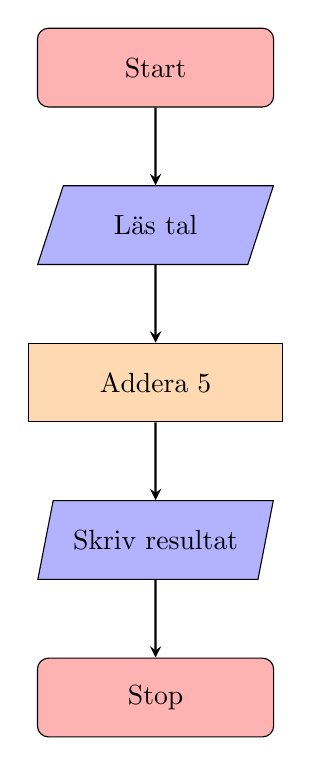
\begin{tikzpicture}[node distance=2cm]
\node (start) [startstop] {Start};
\node (input) [io, below of=start] {Läs tal};
\node (process) [process, below of=input] {Addera 5};
\node (output) [io, below of=process] {Skriv resultat};
\node (stop) [startstop, below of=output] {Stop};

\draw [arrow] (start) -- (input);
\draw [arrow] (input) -- (process);
\draw [arrow] (process) -- (output);
\draw [arrow] (output) -- (stop);
\end{tikzpicture}
}
&

% Python-kod
\raggedright
\begin{lstlisting}[xleftmargin=1.5em]
# Läs ett tal från användaren
nummer = int(input("Ange ett tal: "))

# Lägg till 5
resultat = nummer + 5

# Skriv ut resultatet
print("Resultatet är:", resultat)
\end{lstlisting}
\vspace{0.5em}
Enkelt program som läser in ett tal från användaren, adderar 5 till det, och skriver ut resultatet igen.
\\
\end{tabular*}


\subsection*{Exempel 2: Beslutsstruktur}
\begin{tabular*}{\linewidth}{@{\extracolsep{\fill}} p{0.45\linewidth} | p{0.5\linewidth}}
\textbf{Flödesdiagram:} & \textbf{Python-kod:} \\
\hline

% Flödesdiagram
\raisebox{-\totalheight}{%
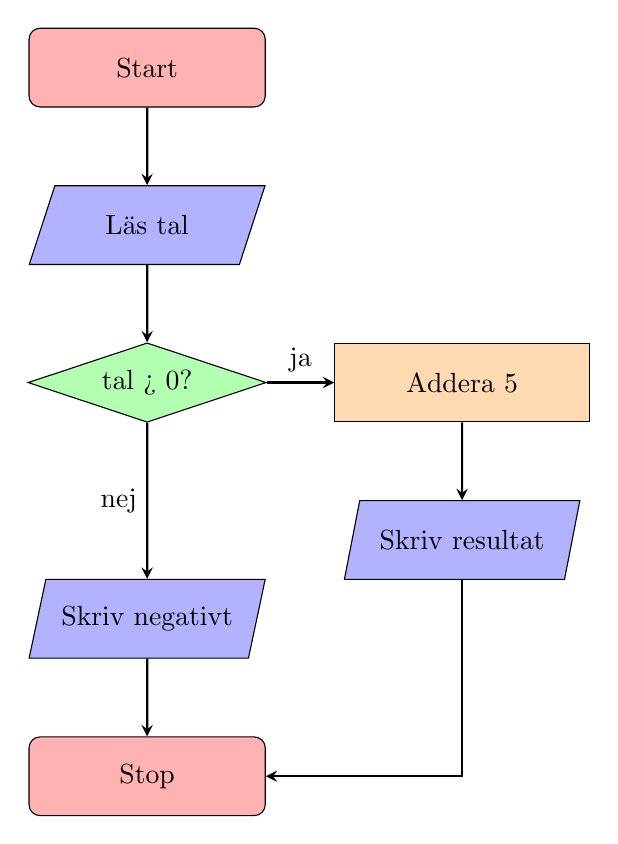
\begin{tikzpicture}[node distance=2cm]
\node (start) [startstop] {Start};
\node (input) [io, below of=start] {Läs tal};
\node (decision) [decision, below of=input] {tal > 0?};
\node (process) [process, right of=decision,xshift=2cm] {Addera 5};
\node (output1) [io, below of=process] {Skriv resultat};
\node (output2) [io, below of=decision, yshift=-1cm] {Skriv negativt};
\node (stop) [startstop, below of=output2] {Stop};

\draw [arrow] (start) -- (input);
\draw [arrow] (input) -- (decision);
\draw [arrow] (decision.east) -- node[anchor=south] {ja} (process.west);
\draw [arrow] (process) -- (output1);
\draw [arrow] (decision.south) -- node[anchor=east] {nej} (output2.north);
\draw [arrow] (output1.south) |- (stop.east);
\draw [arrow] (output2) -- (stop);
\end{tikzpicture}
}
&

% Python-kod
\raggedright
\begin{lstlisting}[xleftmargin=1.5em]
# Läs ett tal från användaren
nummer = int(input("Ange ett tal: "))

if nummer > 0:
    # Addera 5 om talet är positivt
    resultat = nummer + 5
    print("Resultatet är:", resultat)
else:
    # Annars skriv "negativt"
    print("Talet är negativt")
\end{lstlisting}
\vspace{0.5em}
Användaren skriver in ett tal. Om det är större än 0 adderas fem till talet, och resultatet skrivs ut.
Annars skrivs endast ut att talet är negativt utan att addera något.
\\
\end{tabular*}


\subsection*{Exempel 3: While-loop med villkor}
\begin{tabular*}{\linewidth}{@{\extracolsep{\fill}} p{0.55\linewidth} | p{0.45\linewidth}}
\textbf{Flödesdiagram:} & \textbf{Python-kod:} \\
\hline

% Flödesdiagram
\raisebox{-\totalheight}{%
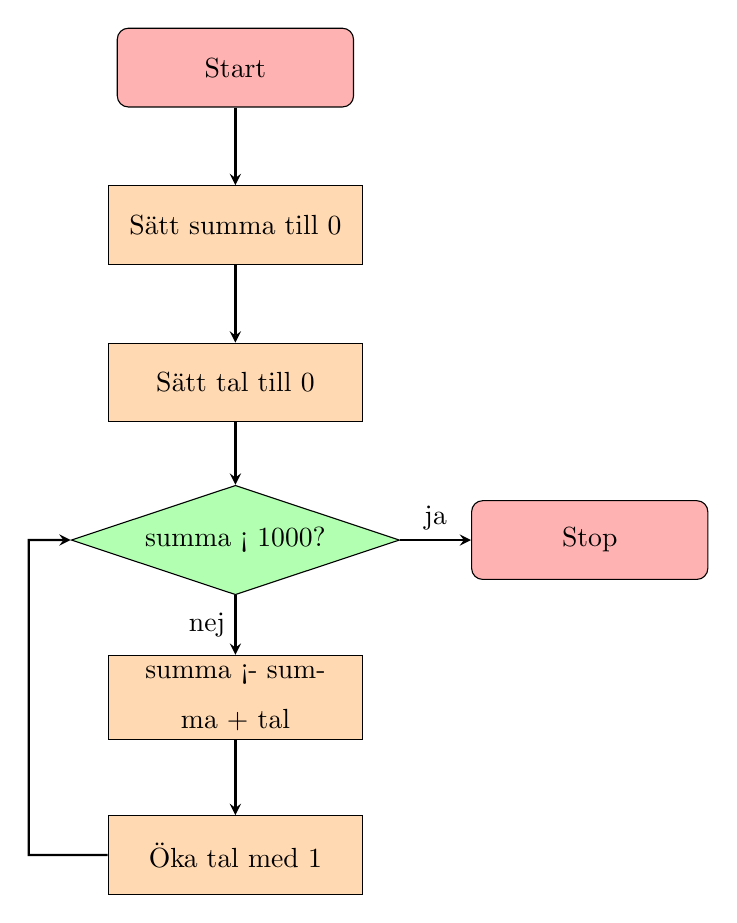
\begin{tikzpicture}[node distance=2cm]
\node (start) [startstop] {Start};
\node (summainit) [process, below of=start] {Sätt summa till 0};
\node (talinit) [process, below of=summainit] {Sätt tal till 0};
\node (decision) [decision, below of=talinit] {summa < 1000?};
\node (summera) [process, below of=decision] {summa <- summa + tal};
\node (ökatal) [process, below of=summera] {Öka tal med 1};
\node (stop) [startstop, right of=decision, xshift=2.5cm] {Stop};

\draw [arrow] (start) -- (summainit);
\draw [arrow] (summainit) -- (talinit);
\draw [arrow] (talinit) -- (decision);
\draw [arrow] (decision.east) -- node[anchor=south] {ja} (stop.west);
\draw [arrow] (decision.south) -- node[anchor=east] {nej} (summera);
\draw [arrow] (summera) -- (ökatal);
\draw [arrow] (ökatal.west) -- ++(-1,0) -- ++(0,4) -- (decision.west);

%\draw [arrow] (ökatal) -- (decision.west);

\end{tikzpicture}
}
&

% Python-kod
\raggedright
\begin{lstlisting}[caption={Summera positiva tal}, xleftmargin=1.5em]
# Räknar 1+2+3+4+5... så länge summan är mindre än 1000
summa = 0
tal = 1
while summa < 1000:
    summa = summa + tal

print("Summa 1+2+3+...+",tal,">1000")

\end{lstlisting}
\vspace{0.5em}
Räknar ut vilket tal vi behöver räkna till så att $1+2+3+\cdots+tal>1000$.
\\
\end{tabular*}
\newpage
\subsection*{Exempel 4: Kombinerad if-sats och while-loop}
\begin{tabular*}{\linewidth}{@{\extracolsep{\fill}} p{0.55\linewidth} | p{0.48\linewidth}}
\textbf{Flödesdiagram:} & \textbf{Python-kod:} \\
\hline

% Flödesdiagram
\raisebox{-\totalheight}{%
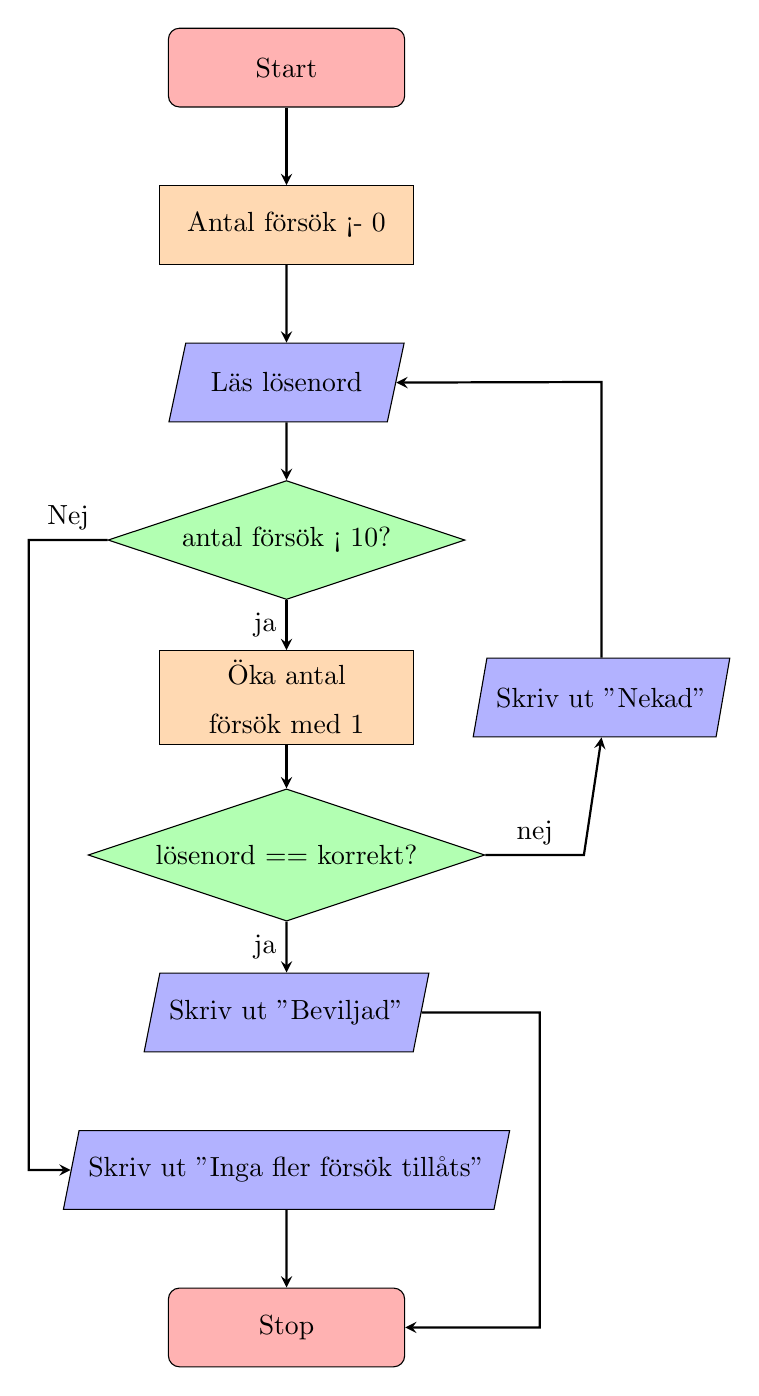
\begin{tikzpicture}[node distance=2cm]
\node (start) [startstop] {Start};
\node (antalinit) [process, below of=start] {Antal försök <- 0};

\node (input) [io, below of=antalinit] {Läs lösenord};
\node (decision1) [decision, below of=input] {antal försök < 10?};
\node (antalöka) [process, below of=decision1] {Öka antal försök med 1};

\node (decision2) [decision, below of=antalöka] {lösenord == korrekt?};
\node (denied) [io, right of=antalöka, xshift=2cm] {Skriv ut ''Nekad''};
\node (access) [io, below of=decision2] {Skriv ut ''Beviljad''};
\node (maxtries) [io, below of=access] {Skriv ut ''Inga fler försök tillåts''};


\node (stop) [startstop, below of=maxtries] {Stop};

\draw [arrow] (start) -- (antalinit);
\draw [arrow] (antalinit) -- (input);
\draw [arrow] (input) -- (decision1);
\draw [arrow] (decision1.south) -- node[anchor=east] {ja} (antalöka.north);

\draw [arrow] (antalöka) -- (decision2);
\draw [arrow] (decision2.south) -- node[anchor=east] {ja} (access.north);

\draw [arrow] (decision1.west) -- node[anchor=south] {Nej} ++(-1,0) -- ++(0,-8) -- (maxtries.west);
\draw [arrow] (maxtries) -- (stop);

\draw [arrow] (access.east) -- ++(1.5,0) -- ++(0,-4) -- (stop.east);


\draw [arrow] (denied.north) -- ++(0,3.5) -- (input.east);
\draw [arrow] (decision2.east) -- node[anchor=south] {nej} ++(1.25,0) -- (denied.south);


\end{tikzpicture}
}
&

% Python-kod
\raggedright
\begin{lstlisting}[xleftmargin=1.5em]
# Enkel lösenordskontroll
korrekt_losenord = "python123"
antal_försök=0

while antal_försök<10:
    losenord = input("Ange lösenord: ")
    if losenord == korrekt_losenord:
        print("Beviljad!")
        break
    else:
        print("Nekad")
    antal_försök = antal_försök + 1
if antal_försök == 10:
  print("Inga fler försök tillåts")
\end{lstlisting}
\vspace{0.5em}
Låter användaren mata in ett lösenord tills dess att användaren skriver in
''python123''. Programmet skriver ut meddelanden vid varje försök som säger
om lösenordet var rätt eller inte. Programmet ger max 10 försök till användaren.
Notera att i flödesdiagrammet finns ingen direkt motsvarighet till if-satsen efter loopen.
Det beror på att flödesdiagramet beskriver vad programmet gör logiskt och inte i en direktöversättning. 
Eftersom loopen i flödesdiagramet avslutas genom \textbf{Antal försök > 10?} behövs inte en extra koll.
\\
\end{tabular*}


\newpage
\section{Kodexempel: Logiska uttryck och booleanska värden}
\label{examples:boolean}
\exToSecRef{section:boolean}
\subsection*{Datatypen \texttt{bool}}

\begin{lstlisting}[title=Exempel 1: Sanna och falska värden]
# Booleanska värden är antingen True eller False
a = True
b = False
print("a är:", a)
print("b är:", b)
\end{lstlisting}

\begin{lstlisting}[title=Exempel 2: Booleanska värden från jämförelser]
# Jämförelser returnerar ett booleskt värde
print(5 > 3)   # True
print(10 < 7)  # False
print(3 == 3)  # True
print(4 != 5)  # True
\end{lstlisting}

\subsection*{Logiska operatorer: and, or, not}

\begin{lstlisting}[title=Exempel 3: Använda \texttt{and}]
# and returnerar True om båda villkoren är sanna
print(True and True)    # True
print(True and False)   # False
print(5 > 3 and 2 < 4)  # True
print(5 > 3 and 2 > 4)  # False
\end{lstlisting}

\begin{lstlisting}[title=Exempel 4: Använda \texttt{or}]
# or returnerar True om minst ett villkor är sant
print(True or False)    # True
print(False or False)   # False
print(5 > 3 or 2 > 4)   # True
print(10 < 7 or 1 == 1) # True
\end{lstlisting}

\begin{lstlisting}[title=Exempel 5: Använda \texttt{not}]
# not inverterar ett booleskt värde
print(not True)   # False
print(not False)  # True
print(not (5 > 3)) # False
\end{lstlisting}

\subsection*{Kombination av logiska uttryck}

\begin{lstlisting}[title=Exempel 6: Kombinera and\, or och not]
# Kombinera flera logiska operatorer
x = 10
y = 5
print((x > y) and (y > 2))    # True
print((x > y) or (y < 2))     # True
print(not (x == y))           # True
\end{lstlisting}

\begin{lstlisting}[title=Exempel 7: Operatorns prioritet]
# not har högre prioritet än and/or
print(not True and False)  # False
print(not (True and False)) # True
print(True or not False)    # True
print((True or False) and not False) # True
\end{lstlisting}

\subsection*{Vanliga misstag}

\begin{lstlisting}[title=Exempel 8: Glöm inte parenteser vid komplexa uttryck]
x = 10
y = 5

# Fel: operatorprioritet ger oväntat resultat
print(not x > y and y < 2)  # Detta är False

# Rätt: använd parenteser för tydlighet
print((not (x > y)) and (y < 2))  # Detta är True
\end{lstlisting}

\begin{lstlisting}[title=Exempel 9: Jämför inte direkt med \texttt{True}/\texttt{False}]
x = (5 > 3)

# Onödigt sätt
if x == True:
    print("x är sant!")

# Bättre sätt
if x:
    print("x är sant!")
\end{lstlisting}

\subsection*{Exempel i praktisk användning}

\begin{lstlisting}[title=Exempel 10: Kontrollera tillgång till system]
# Villkor: Användaren måste vara inloggad och ha adminrättigheter
inloggad = True
admin = False

if inloggad and admin:
    print("Välkommen, admin!")
else:
    print("Åtkomst nekad.")
\end{lstlisting}

\begin{lstlisting}[title=Exempel 11: Kontrollera om ett tal är i intervall]
# Kontrollera om ett tal är mellan 10 och 20
tal = 15

if tal >= 10 and tal <= 20:
    print("Talet är inom intervallet.")
else:
    print("Talet är utanför intervallet.")
\end{lstlisting}

\newpage
\section{Kodexempel: Matematik i Python}
\label{examples:math}
\exToSecRef{section:math}
\subsection*{\texttt{math}-modulen}

\begin{lstlisting}[title=Exempel 1: Importera math-modulen]
# För att använda funktioner från math-modulen måste vi importera den
import math

# Exempel: Beräkna kvadratroten av ett tal
tal = 25
resultat = math.sqrt(tal)
print("Kvadratroten av", tal, "är", resultat)
\end{lstlisting}

\begin{lstlisting}[title=Exempel 2: Exponentiering med \texttt{math.pow()}]
import math

# math.pow() beräknar bas upphöjt till exponent
bas = 2
exponent = 3
resultat = math.pow(bas, exponent)
print(bas, "upphöjt till", exponent, "är", resultat)
\end{lstlisting}

\begin{lstlisting}[title=Exempel 3: Heltalsavrundning med \texttt{math.floor()} och \texttt{math.ceil()}]
import math

# math.floor() rundar ner till närmaste heltal
print(math.floor(5.7))  # 5

# math.ceil() rundar upp till närmaste heltal
print(math.ceil(5.7))   # 6
\end{lstlisting}

\begin{lstlisting}[title=Exempel 4: Använda matematiska konstanter som \texttt{math.pi}]
import math

# math.pi är ett konstant värde för pi
radie = 5
omkrets = 2 * math.pi * radie
print("Omkretsen av en cirkel med radie", radie, "är", omkrets)
\end{lstlisting}

\subsection*{Specialoperationer}

\begin{lstlisting}[title=Exempel 5: Exponentiering med \texttt{**}]
# Operatorn ** används för att beräkna potenser
bas = 3
exponent = 4
resultat = bas ** exponent
print(bas, "upphöjt till", exponent, "är", resultat)  # 81
\end{lstlisting}

\begin{lstlisting}[title=Exempel 6: Modulusoperatorn \texttt{\%}]
# Modulus operatorn \% beräknar resten av en division
a = 10
b = 3
rest = a % b
print("Resten av", a, "delat med", b, "är", rest)  # 1
\end{lstlisting}

\begin{lstlisting}[title=Exempel 7: Heltalsdivision med \texttt{//}]
# Heltalsdivision returnerar endast heltalsdelen av resultatet
a = 10
b = 3
kvot = a // b
print(a, "heltalsdividerat med", b, "är", kvot)  # 3
\end{lstlisting}

\subsection*{Kombinerade exempel}

\begin{lstlisting}[title=Exempel 8: Beräkna hypotenusan i en triangel]
import math

# Pythagoras sats: c = sqrt(a^2 + b^2)
a = 3
b = 4
c = math.sqrt(a**2 + b**2)
print("Hypotenusan för en triangel med sidorna", a, "och", b, "är", c)  # 5.0
\end{lstlisting}

\begin{lstlisting}[title=Exempel 9: Kontrollera om ett tal är jämnt eller udda]
# Modulus kan användas för att kontrollera jämnhet
tal = 15
if tal % 2 == 0:
    print(tal, "är ett jämnt tal.")
else:
    print(tal, "är ett udda tal.")
\end{lstlisting}

\begin{lstlisting}[title=Exempel 10: Rundning av tal till närmaste heltal]
import math

# Kombinera floor och ceil för att göra en egen rundningsfunktion
tal = 5.5

if tal - math.floor(tal) < 0.5:
    avrundat = math.floor(tal)
else:
    avrundat = math.ceil(tal)

print("Rundning av", tal, "ger", avrundat)  # 6
\end{lstlisting}

\begin{lstlisting}[title=Exempel 11: Area av en cirkel]
import math

# Beräkna area av en cirkel
radie = 7
area = math.pi * radie**2
print("Arean av en cirkel med radie", radie, "är", area)
\end{lstlisting}

\newpage
\section{Kodexempel: Bubble Sort}
\label{examples:bubblesort}
\exToSecRef{section:bubblesort}
\subsection*{Exempel 1: Grundläggande Bubble Sort-algoritm}

\begin{lstlisting}[title=Bubble Sort - Grundläggande implementation]
def bubble_sort(lista):
    n = len(lista)
    for i in range(n):
        for j in range(0, n - i - 1):
            if lista[j] > lista[j + 1]:
                # Byt plats om elementet är större än det nästa
                lista[j], lista[j + 1] = lista[j + 1], lista[j]

# Testa med en lista
tal_lista = [64, 34, 25, 12, 22, 11, 90]
bubble_sort(tal_lista)
print("Sorterad lista:", tal_lista)
# Output: Sorterad lista: [11, 12, 22, 25, 34, 64, 90]
\end{lstlisting}

\subsection*{Exempel 2: Visualisering av varje steg i sorteringen}

\begin{lstlisting}[title=Bubble Sort - Visualisering av stegen]
def bubble_sort_med_steg(lista):
    n = len(lista)
    for i in range(n):
        print(f"Pass {i + 1}: {lista}")  # Visa listan vid varje pass
        for j in range(0, n - i - 1):
            if lista[j] > lista[j + 1]:
                lista[j], lista[j + 1] = lista[j + 1], lista[j]

tal_lista = [5, 3, 8, 6]
bubble_sort_med_steg(tal_lista)
# Output:
# Pass 1: [5, 3, 8, 6]
# Pass 2: [3, 5, 6, 8]
# Pass 3: [3, 5, 6, 8]
# Pass 4: [3, 5, 6, 8]
\end{lstlisting}

\subsection*{Exempel 3: Optimera Bubble Sort med tidig avbrytning}

\begin{lstlisting}[title=Bubble Sort - Optimerad version]
def bubble_sort_optimerad(lista):
    n = len(lista)
    for i in range(n):
        bytt = False
        for j in range(0, n - i - 1):
            if lista[j] > lista[j + 1]:
                lista[j], lista[j + 1] = lista[j + 1], lista[j]
                bytt = True
        if not bytt:
            break  # Avbryt om listan redan är sorterad

tal_lista = [1, 2, 3, 4, 5]
bubble_sort_optimerad(tal_lista)
print("Sorterad lista:", tal_lista)
# Output: Sorterad lista: [1, 2, 3, 4, 5]
\end{lstlisting}

\subsection*{Exempel 4: Bubble Sort på strängar}

\begin{lstlisting}[title=Bubble Sort - Sortera strängar]
def bubble_sort(lista):
    n = len(lista)
    for i in range(n):
        for j in range(0, n - i - 1):
            if lista[j] > lista[j + 1]:
                lista[j], lista[j + 1] = lista[j + 1], lista[j]

sträng_lista = ["banan", "äpple", "citron", "druva"]
bubble_sort(sträng_lista)
print("Sorterad lista:", sträng_lista)
# Output: Sorterad lista: ['äpple', 'banan', 'citron', 'druva']
\end{lstlisting}

\subsection*{Exempel 5: Praktisk användning av Bubble Sort}

\begin{lstlisting}[title=Bubble Sort - Praktisk användning]
# Sortera elever baserat på deras poäng
elever = [("Anna", 85), ("Björn", 75), ("Cecilia", 90), ("David", 80)]

def bubble_sort(lista):
    n = len(lista)
    for i in range(n):
        for j in range(0, n - i - 1):
            if lista[j][1] > lista[j + 1][1]:  # Sortera efter poäng
                lista[j], lista[j + 1] = lista[j + 1], lista[j]

bubble_sort(elever)
print("Sorterade elever:", elever)
# Output: Sorterade elever: [('Björn', 75), ('David', 80), ('Anna', 85), ('Cecilia', 90)]
\end{lstlisting}

\subsection*{Tips och rekommendationer}
- Bubble Sort är enkel att förstå och implementera, men ineffektiv för stora datamängder.
- Använd optimerad version för att förbättra prestanda om listan kan vara delvis sorterad.

\newpage
\section{Kodexempel: Linjär och Binär Sökning}
\label{examples:search}
\exToSecRef{section:search}
\subsection*{Exempel 1: Linjär sökning i en lista}

\begin{lstlisting}[title=Linjär sökning i en lista]
def linjar_sokning(lista, mål):
    for index, värde i enumerate(lista):
        if värde == mål:
            return index  # Returnera index om målet hittas
    return -1  # Returnera -1 om målet inte finns

tal_lista = [10, 20, 30, 40, 50]
mål = 30
resultat = linjar_sokning(tal_lista, mål)
print(f"Elementet finns vid index: {resultat}")
# Output: Elementet finns vid index: 2
\end{lstlisting}

\subsection*{Exempel 2: Linjär sökning i en dictionary}

\begin{lstlisting}[title=Linjär sökning i en dictionary]
elever = {"Anna": 85, "Björn": 75, "Cecilia": 90, "David": 80}

def linjar_sokning_dict(dictionary, mål):
    for nyckel, värde i dictionary.items():
        if värde == mål:
            return nyckel
    return None

mål = 90
resultat = linjar_sokning_dict(elever, mål)
print(f"Eleven med poäng {mål} är: {resultat}")
# Output: Eleven med poäng 90 är: Cecilia
\end{lstlisting}

\subsection*{Exempel 3: Binär sökning i en sorterad lista}

\begin{lstlisting}[title=Binär sökning i en sorterad lista]
def binar_sokning(lista, mål):
    vänster, höger = 0, len(lista) - 1
    while vänster <= höger:
        mitten = (vänster + höger) // 2
        if lista[mitten] == mål:
            return mitten
        elif lista[mitten] < mål:
            vänster = mitten + 1
        else:
            höger = mitten - 1
    return -1

tal_lista = [10, 20, 30, 40, 50]
mål = 40
resultat = binar_sokning(tal_lista, mål)
print(f"Elementet finns vid index: {resultat}")
# Output: Elementet finns vid index: 3
\end{lstlisting}

\subsection*{Exempel 4: Visualisering av binär sökning}

\begin{lstlisting}[title=Binär sökning - Visualisering]
def binar_sokning_visualisering(lista, mål):
    vänster, höger = 0, len(lista) - 1
    steg = 0
    while vänster <= höger:
        mitten = (vänster + höger) // 2
        print(f"Steg {steg}: Vänster={vänster}, Höger={höger}, Mitten={mitten}")
        if lista[mitten] == mål:
            return mitten
        elif lista[mitten] < mål:
            vänster = mitten + 1
        else:
            höger = mitten - 1
        steg += 1
    return -1

tal_lista = [10, 20, 30, 40, 50]
mål = 40
binar_sokning_visualisering(tal_lista, mål)
# Output:
# Steg 0: Vänster=0, Höger=4, Mitten=2
# Steg 1: Vänster=3, Höger=4, Mitten=3
# Output: Elementet finns vid index: 3
\end{lstlisting}

\subsection*{Exempel 5: Tidskomplexitet}

\begin{rconceptbox}{Tidskomplexitet för sökning}{
\textbf{Linjär sökning:} $O(n)$, där $n$ är antalet element i listan.\\
\textbf{Binär sökning:} $O(\log n)$, men listan måste vara sorterad.
}
\end{rconceptbox}

\subsection*{Exempel 6: Binär sökning med rekursion}

\begin{lstlisting}[title=Binär sökning - Rekursiv implementation]
def binar_sokning_rekursiv(lista, mål, vänster, höger):
    if vänster > höger:
        return -1
    mitten = (vänster + höger) // 2
    if lista[mitten] == mål:
        return mitten
    elif lista[mitten] < mål:
        return binar_sokning_rekursiv(lista, mål, mitten + 1, höger)
    else:
        return binar_sokning_rekursiv(lista, mål, vänster, mitten - 1)

tal_lista = [10, 20, 30, 40, 50]
mål = 50
resultat = binar_sokning_rekursiv(tal_lista, mål, 0, len(tal_lista) - 1)
print(f"Elementet finns vid index: {resultat}")
# Output: Elementet finns vid index: 4
\end{lstlisting}

\subsection*{Praktiska tips}
- Linjär sökning fungerar för osorterade listor eller dictionaries.
- Binär sökning kräver en sorterad lista och är betydligt snabbare för större datamängder.

\newpage
\section{Kodexempel: Pseudokod}
\label{examples:psuedocode}
\exToSecRef{section:psuedocode}
\subsection*{Exempel 1: Summera tal i en lista}

\textbf{Pseudokod:}
\begin{verbatim}
START
  Lista = [10, 20, 30, 40]
  SUMMA = 0
  FOR varje TAL i Lista
    SUMMA = SUMMA + TAL
  END FOR
  Skriv SUMMA
END
\end{verbatim}

\textbf{Python-kod:}
\begin{lstlisting}[title=Summera tal i en lista]
tal_lista = [10, 20, 30, 40]
summa = 0

for tal in tal_lista:
    summa += tal

print(f"Summan är: {summa}")
# Output: Summan är: 100
\end{lstlisting}

\subsection*{Exempel 2: Kontrollera om ett tal är jämnt}

\textbf{Pseudokod:}
\begin{verbatim}
START
  Läs in TAL
  IF TAL modulo 2 = 0 THEN
    Skriv "Talet är jämnt"
  ELSE
    Skriv "Talet är udda"
  END IF
END
\end{verbatim}

\textbf{Python-kod:}
\begin{lstlisting}[title=Kontrollera om ett tal är jämnt]
tal = int(input("Ange ett tal: "))

if tal % 2 == 0:
    print("Talet är jämnt")
else:
    print("Talet är udda")
# Testa med tal som 4 och 7
\end{lstlisting}

\subsection*{Exempel 3: Hitta det största talet i en lista}

\textbf{Pseudokod:}
\begin{verbatim}
START
  Lista = [12, 45, 23, 89]
  MAX = Lista[0]
  FOR varje TAL i Lista
    IF TAL > MAX THEN
      MAX = TAL
    END IF
  END FOR
  Skriv MAX
END
\end{verbatim}

\textbf{Python-kod:}
\begin{lstlisting}[title=Hitta det största talet i en lista]
tal_lista = [12, 45, 23, 89]
största_talet = tal_lista[0]

for tal in tal_lista:
    if tal > största_talet:
        största_talet = tal

print(f"Det största talet är: {största_talet}")
# Output: Det största talet är: 89
\end{lstlisting}

\subsection*{Exempel 4: Beräkna fakultet av ett tal}

\textbf{Pseudokod:}
\begin{verbatim}
START
  Läs in TAL
  PRODUKT = 1
  FOR i = 1 TILL TAL
    PRODUKT = PRODUKT * i
  END FOR
  Skriv PRODUKT
END
\end{verbatim}

\textbf{Python-kod:}
\begin{lstlisting}[title=Beräkna fakultet av ett tal]
tal = int(input("Ange ett tal: "))
fakultet = 1

for i in range(1, tal + 1):
    fakultet *= i

print(f"Fakulteten av {tal} är: {fakultet}")
# Testa med 5 (output: 120)
\end{lstlisting}

\subsection*{Exempel 5: Fibonaccital (Iterativt)}

\textbf{Pseudokod:}
\begin{verbatim}
START
  Läs in N
  A = 0
  B = 1
  FOR i = 1 TILL N
    Skriv A
    TEMP = A + B
    A = B
    B = TEMP
  END FOR
END
\end{verbatim}

\textbf{Python-kod:}
\begin{lstlisting}[title=Fibonaccital - Iterativ metod]
n = int(input("Hur många Fibonaccital vill du visa? "))
a, b = 0, 1

for _ in range(n):
    print(a, end=" ")
    a, b = b, a + b
# Testa med 7 (output: 0 1 1 2 3 5 8)
\end{lstlisting}

\newpage
\section{Kodexempel: Rekursion}
\label{examples:recursion}
\exToSecRef{section:recursion}
\subsection*{Exempel 1: Rekursionens grunder}

En rekursiv funktion anropar sig själv för att lösa mindre delar av ett problem. En rekursiv funktion måste innehålla:
- Ett \textbf{basfall} som avslutar rekursionen.
- Ett \textbf{rekursivt fall} som löser problemet genom att anropa sig själv.

\textbf{Exempel på rekursiv nedräkning:}
\begin{lstlisting}[title=Nedräkning med rekursion]
def countdown(n):
    if n == 0:  # Basfall
        print("Klar!")
    else:  # Rekursivt fall
        print(n)
        countdown(n - 1)

countdown(5)
# Output: 5 4 3 2 1 Klar!
\end{lstlisting}

\subsection*{Exempel 2: Faktorial med rekursion}

Faktorial av ett tal \( n \) definieras som \( n! = n \cdot (n-1) \cdot (n-2) \cdots 1 \).

\textbf{Rekursiv definition:}
\[
\text{faktorial}(n) = 
\begin{cases} 
1 & \text{om } n = 0 \\
n \cdot \text{faktorial}(n-1) & \text{om } n > 0
\end{cases}
\]

\textbf{Python-kod:}
\begin{lstlisting}[title=Faktorial med rekursion]
def faktorial(n):
    if n == 0:  # Basfall
        return 1
    else:  # Rekursivt fall
        return n * faktorial(n - 1)

print(faktorial(5))  # Output: 120
\end{lstlisting}

\subsection*{Exempel 3: Binärsökning med rekursion}

Binärsökning hittar ett element i en sorterad lista genom att dela sökområdet i två delar vid varje steg.

\textbf{Rekursiv algoritm:}
\begin{verbatim}
START
  Om lista är tom: returnera False
  Beräkna mittenindex
  Om nyckel = mitten: returnera True
  Om nyckel < mitten: sök i vänstra halvan
  Om nyckel > mitten: sök i högra halvan
END
\end{verbatim}

\textbf{Python-kod:}
\begin{lstlisting}[title=Binärsökning med rekursion]
def binsok(lista, nyckel, vänster, höger):
    if vänster > höger:  # Basfall
        return False

    mitten = (vänster + höger) // 2

    if lista[mitten] == nyckel:  # Hittat nyckeln
        return True
    elif nyckel < lista[mitten]:  # Sök i vänstra halvan
        return binsok(lista, nyckel, vänster, mitten - 1)
    else:  # Sök i högra halvan
        return binsok(lista, nyckel, mitten + 1, höger)

# Testa med en sorterad lista
sorterad_lista = [1, 3, 5, 7, 9, 11]
nyckel = 7
print(binsok(sorterad_lista, nyckel, 0, len(sorterad_lista) - 1))  # Output: True
\end{lstlisting}

\subsection*{Exempel 4: Rekursivt fibonaccital}

Ett exempel som visar rekursiv ineffektivitet:
\begin{lstlisting}[title=Fibonaccital med rekursion]
def fibonacci(n):
    if n <= 1:  # Basfall
        return n
    else:  # Rekursivt fall
        return fibonacci(n - 1) + fibonacci(n - 2)

print(fibonacci(6))  # Output: 8
\end{lstlisting}
\textbf{Observera:} Rekursiva algoritmer som denna kan vara ineffektiva och bör förbättras med memoization eller iteration för stora \( n \).



\end{document}
